\chapter*{Chapter 5}


In \autoref{cpt:chapter_1} we have introduced a new approach where multiple \acfp{VNO}, each providing a different service, can coexist on the same \acp{PON} network while running a virtual instance of the \ac{DBA} algorithm of their choice and aggregating these scheduling decisions into a final \ac{BMap}. Two methods for dealing with the excess bandwidth of the \acp{VNO} namely \textit{Sharing} and \textit{Non-Sharing} were analyzed with the conclusion that the sharing method considerably improves the utilization of the network. Nevertheless, \autoref{cpt:chapter_1} overlooks the incentives of the \acp{VNO} to share their excess bandwidth with other \ac{VNO}'s while it can blindly allocate the bandwidth to its own users' unpredictable demand surge.

In situations that the participants lack incentives for sharing a resource, \textit{monetization} (i.e., monetary compensation) comes to the help as a manifest tool to incentivize self-interested agents to engage in sharing (e.g., ride-sharing and Airbnb). The same tool can be used to address the incentive problem in multi-tenant \acp{PON}. Where the \acp{VNO} are compensated by money/credit in return for sharing their excess capacity with others. The \acp{VNO} in demand of extra capacity will report their valuations while on the other side the \acp{VNO} who own this extra capacity will announce their valuation and then simply, the demander with the highest valuation gets the capacity from the supplier with the lowest. Though, this is an unrealistic over-simplification of the allocation as this solution will in many ways allow the \acp{VNO} to strategize and take advantage of this design flaw and improve their payoff by damaging the others'. In this chapter, we will study the potential design flaws associated with such a market and will try to build a mechanism to minimize or entirely solve them. In the following section we propose a network model for the inter-operator excess capacity sharing in \acp{PON} and introduce the market players and elements along with the monetary interactions among them.


%%%%%%%%%%%%%%%%%%%%%%%%%%%%%%%%%%%%%%%%%%%%%%%%%%%%%%%%%%
%%%%%%%%%%%%%%%%%%%%%%%%%%%%%%%%%%%%%%%%%%%%%%%%%%%%%%%%%%
%%%%%%%%%%%%%%%%%%%%%%%%%SECTION%%%%%%%%%%%%%%%%%%%%%%%%%%
%%%%%%%%%%%%%%%%%%%%%%%%%%%%%%%%%%%%%%%%%%%%%%%%%%%%%%%%%%
%%%%%%%%%%%%%%%%%%%%%%%%%%%%%%%%%%%%%%%%%%%%%%%%%%%%%%%%%%
\section{Market Model}
\label{sec:market-model}
In this section, we present a market model (depicted in \figureautorefname~\ref{Fig_model}) for the multi-tenant \acp{PON} excess capacity market. We first introduce the market players and the preliminaries while defining the essential parameters and features of the market. Next, we point out the desired economic properties of the market and define the utility function of the market players.

\begin{figure*}[htbp]
% \vspace{-3mm}
  \centering
  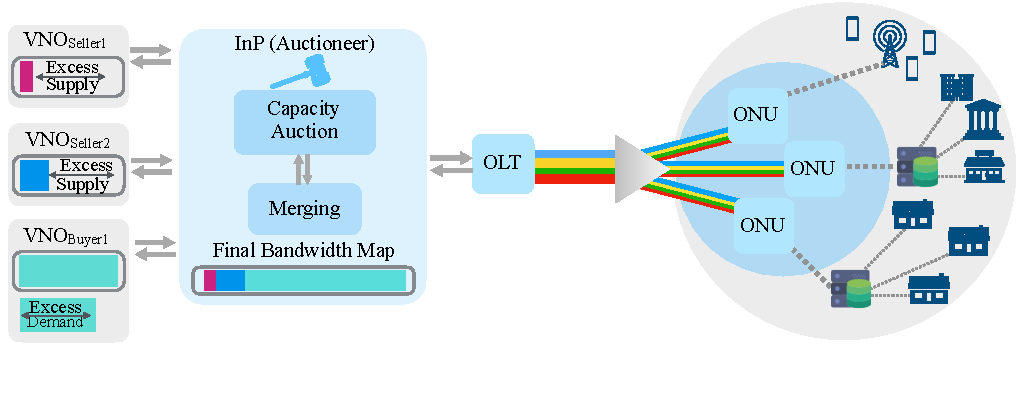
\includegraphics[width=0.9\columnwidth]{Figures/pon.pdf}
% \vspace{-4mm}
\caption{The Multi-Tenant \acp{PON} Network Model}
\label{Fig_model}
% \vspace{-1mm}
\end{figure*}

\subsection{Preliminaries}
The market consists of a set of $M$ sellers $\mathbb{S}=\{s_{1}, s_{2}, ...,s_{i}\}, \ i \in M$ and a set of $N$ buyers $\mathbb{B}=\{b_{1}, b_{2}, ...,b_{j}\}, \ j \in N$ and one auctioneer. This constructs a two-sided market in which a number of traders are competing to trade identical items in a way that it will maximize their payoff. There is also an auction maker (broker) present that is responsible for operating the auction. In our market, the \ac{InP} plays the role of the auctioneer.

The auctioneer initiates the auction. Each seller announces the quantity of the items offered $q^S_{i}$ along with the per-item ask value $v^S_{i}$ to the auctioneer. Simultaneously the buyers will send their pair of the number of items required $q^B_{j}$ and the bid value $v^B_{j}$ to the auctioneer. The ask and bid values ($v^S_{i}, v^B_{j}$) are $\in$ (0, 1). The auction mechanism is common knowledge.

\begin{Definition}
\textbf{\acp{VNO}' Per-Item Valuation}

The valuation of a \ac{VNO} for an item is driven by its probability of being able to utilize it. This valuation thus ranges between [0,1], $p=0$ for definitely not having any user asking for any bandwidth. $p \in (0,1)$ for having a probability between $0$ and $1$ that a new upstream burst arrives in one of the users' buffer since the last time that the buffer occupancy was reported (this might be predicted using machine learning or traffic history monitoring techniques). And $p=1$ for definite demand from the users that in \acp{PON} is referred to as \textit{"buffer occupancy reports"}. For instance, if a \ac{VNO} reports a quantity of 1000 items and its preassigned provisioned share is 900 items, it means that it will certainly utilize the 900 items with the probability of 1 and is demanding for 100 extra items and there is a probability of $v_j$ that it will utilize this item.
\end{Definition}
\begin{table}
    \caption{Market Model Parameters}
    \label{tbl:params}
    \centering
      \begin{tabular}{>{\itshape}ll}
        \toprule
        \upshape Parameter & Descriptions\\\midrule
        $S_i$ & $i^{th}$ Seller\\
        \smallskip
        $B_j$ & $j^{th}$ Buyer\\
        \smallskip
        $v^{\textsc{s}}_{i}$ & Per-item ask value of $i^{th}$ seller\\
        \smallskip
        $v^{\textsc{b}}_{j}$ & Per-item bid value of $j^{th}$ buyer\\
        \smallskip
        $q^{\textsc{s}}_{i}$ & Quantity of the items offered by $i^{th}$ seller\\
        \smallskip
        $q^{\textsc{b}}_{j}$ & Quantity of the items demanded by $j^{th}$ buyer\\
        \smallskip
        $\theta^{\textsc{s}}_{i}$ & Quantity of the items sold by $i^{th}$ seller\\
        \smallskip
        $\theta^{\textsc{b}}_{j}$ & Quantity of the items bought by $j^{th}$ buyer\\
        \smallskip
        $\Theta_{\textsc{p}{\tiny r}}$ & Total No. items traded using the proposed mechanism\\
        \smallskip
        $\Theta_{\textsc{xu}}$ & Total No. items traded using the Xu et al. mechanism\\
        \smallskip
        $p^{\textsc{s}}$ & Sellers' trade price\\
        \smallskip
        $p^{\textsc{b}}$ & Buyers' trade price\\
        \smallskip
        $u^{\textsc{s}}_{i}$ & Trade utility of $i^{th}$ seller\\
        \smallskip
        $u^{\textsc{b}}_{j}$ & Trade utility of $j^{th}$ buyer\\
        \smallskip
        $u^{\textsc{a}{\tiny uc}}$ & Trade utility of the auctioneer\\\bottomrule
      \end{tabular}
    %   \vspace{-4mm}
  \end{table}


The market model parameters are summarized in Table. \ref{tbl:params}. Each seller $S_{i}(i \in I)$ is willing to supply $q^S_{i}$ items for the minimum price of ${v^S_{i}}$. On the other side of the market each buyer $B_{j} (j \in J)$ is willing to buy $q^B_{j}$ items and is willing to pay $v^B_{j}$ for each item at most.

When the auction has ended, the winning sellers will each receive $p^{\textsc{s}} \times \theta_{i}^\textsc{s}$ and the winning buyers will pay $p^{\textsc{b}} \times \theta_{j}^\textsc{b}$ with the $p^{\textsc{s}}$ and $p^{\textsc{b}}$ as the buyers' and the sellers' trade price and $\theta_{i}^\textsc{s}$ and $\theta_{j}^\textsc{b}$ as the quantity of the items traded for the buyers and the sellers respectively. By our design the traders can be partially satisfied that is they can buy/sell $\theta_i^S \leq q_i^S$ or $\theta_j^B \leq q_j^B$.
% The auctioneer forms a vector of Seller's values (asks) ${V}^S=\{{v^S_1}, {v^S_2}, ..., {v^S_n}\}$ and a vector of buyer's values (bids) ${V}^B=\{{v^B_1}, {v^B_2}, ..., {v^B_m}\}$.

\begin{Definition}
\label{def_strategy}
\textbf{Strategy} 

In the context of our market the only effects that a trader can have on the market, and the final allocation are its reported value and quantity. Thus a trader's strategy is the value and quantity pair that it reports to the auctioneer.
\end{Definition}
A trader can either report its true or a manipulated value which to elaborate further; it can follow a function that maximizes its payoff. All the traders are driven by their payoffs; this current practice may also endanger the market maker's revenue in the long run.

The quantity of items sold/bought by each seller/buyer is shown as $\theta_i^S, \theta_j^B$ respectively. The total number of items traded in the auction ($\Theta$) is calculated as follows:
\begin{equation}
\label{Thetha}
\Theta = \sum_{i=1}^{M} \theta_i^S = \sum_{j=1}^{N} \theta_j^B
\end{equation}
Where $M$ and $N$ are the number of Sellers and buyers respectively.

\subsection{Utility (Payoff)}
% If the mechanism is \ac{IC} it means that we have access to the true valuation of the traders thus it is possible to elicit the amount of utility they gain in the auction. 
The utility of a seller ($u_{i}^\textsc{s}$) is the difference between the total amount paid to them in return for the sold items and their true valuation times the number of items sold ($\Theta_{i}^\textsc{s}$):
\begin{equation}
\label{seller_utility_formula}
u_{i}^\textsc{s} = {\theta_{i}^\textsc{s}}  \times (p^\textsc{s} - {v_{i}^\textsc{s}})
\end{equation}
The utility of a Buyer ($u_{j}^\textsc{b}$) represents the difference between its true valuation for all the acquired items and the its total payment times the number of items acquired ($\Theta_{j}^\textsc{b}$):
\begin{equation}
\label{buyer-utility-formula}
u_{j}^\textsc{b} = {\theta_{j}^\textsc{b}}  \times ({v_{j}^\textsc{b}}-p^\textsc{b})
\end{equation}
The utility of the auctioneer is the budget surplus which is the difference between the amount paid by the buyers and the amount to be paid to the sellers:
\begin{equation}
\label{util-auc}
u^{Auc} = (p^\textsc{b} \times \sum_{i=1}^{M} \theta_i^S) - (p^\textsc{s} \times \sum_{j=1}^{N} \theta_j^B)
\end{equation}
and since according to Eq.\ref{Thetha}
\begin{eqnarray*}
\Theta = \sum_{i=1}^{M} \theta_i^S = \sum_{j=1}^{N} \theta_j^B
% \cos 2\theta & = & \cos^2 \theta - \sin^2 \theta \\
%              & = & 2 \cos^2 \theta - 1.
\end{eqnarray*}
Hence:
\begin{eqnarray}
u^{Auc} = (p^\textsc{b} - p^\textsc{s}) \times \Theta
\end{eqnarray}
% The social welfare is the aggregate utility of all the market playes:
% \begin{equation}
% SW = U^{InP} + U^S + U^B
% \end{equation}



% \subsection{Incentive Compatibility (IC)}
% \subsection{Budget Balance(BB)}
% \subsection{Individual Rationality (IR)}
% \subsection{Allocative Efficiency}

% How to measure the outcome?
% 1- economic-robustness
% 2- Link utilization
% 3- social welfare





% \chapter{Mechanism Design} % Main chapter title
% \label{Chap:Mechanism}


In the next section we propose an auction mechanism that determines the quantity and the price of trade for each trader in a way that first, it requires minimal communication among the trades and the auctioneer while second, it achieves higher or at worst the same social welfare for the market.
%%%%%%%%%%%%%%%%%%%%%%%%%%%%%%%%%%%%%%%%%%%%%%%%%%%%%%%%%%
%%%%%%%%%%%%%%%%%%%%%%%%%%%%%%%%%%%%%%%%%%%%%%%%%%%%%%%%%%
%%%%%%%%%%%%%%%%%%%%%%%%%SECTION%%%%%%%%%%%%%%%%%%%%%%%%%%
%%%%%%%%%%%%%%%%%%%%%%%%%%%%%%%%%%%%%%%%%%%%%%%%%%%%%%%%%%
%%%%%%%%%%%%%%%%%%%%%%%%%%%%%%%%%%%%%%%%%%%%%%%%%%%%%%%%%%

% \section{VCG Based Auction Mechanism}
% \subsection{The Mechanism}
% The auction consists of a set of $M=\{m_{1}, m_{2}, ...,m_{i}\}$ sellers (VNOs with excess capacity) and a set of $N=\{n_{1}, n_{2}, ...,n_{j}\}$ buyers (VNOs with excess demand) and one auctioneer (the InP). We consider an XGS-PON \cite{G.9807.1} with 10-Gbps symmetrical capacity in both upstream and downstream. We define the item to be traded in the auction as the most granular frame unit FU in an XGS-PON. This means for an upstream line rate of 9.953,28-Gbps each FU is one block (16 bytes) according to the XGS-PON standard. Thus, each XGS-PON frame (125 microseconds) can at most contain 9720 allocation structures. i.e., 9,720 FUs per frame.

% The seller ${VNO_{i}}^S$ and the buyer ${VNO^B_{j}}$'s true value is given by ${v^S_{i,FU}}$ and ${v^B_{j,FU}}$ respectively.
% The natural objective of the auction is to buy the items from the sellers with the lowest ${v^S_{i,FU}}$ and sell it to the buyers with the highest ${v^B_{j,FU}}$. This way the revenue generated by the frame will be maximized, i.e., the FUs will be taken from the \acp{VNO} with the lowest probability of utilizing them and will be allocated to the \acp{VNO} with the highest.

% The auction starts by all the \acp{VNO} announcing their per unit valuation for the frame along with the quantity of the excess or demanded FUs. The number of excess FUs of each seller \ac{VNO} is shown by ${q^S_{i}}$ and the number of demanded FUs of the buyer \acp{VNO} is shown by ${q^B_{j}}$.

% After receiving the information from the VNOs, first, the \ac{InP} checks the validity of the auction, i.e., if there are at least one seller and one buyer eligible for efficient trade. If the auction is valid, the \ac{InP} will remove the buyers with a value lower than the lowest value of the sellers and likewise for the sellers with a valuation higher than the highest of the buyers' values. This is due to the fact that the primary objective of the auction is to sell the items to the \acp{VNO} which value it the most and selling the item to a buyer that values it less than all of the sellers will not be acceptable. The same applies to removing the sellers since it will not be acceptable to sell an item to a buyer who values it less than the seller.
% We assume the auctioneer (InP) faithfully executes its duty and all participants unconditionally trust him. We also consider that all the items to be sold (FUs) are identical and indistinguishable, and no buyer prefers one seller's item over that of another.

% The \ac{InP} sets a fixed $BasePrice$ for each FU and admits the FUs from the seller with ${v^S_{i,FU}}$ lower than the $BasePrice$ up to the value $Q^{B}_{N} = \sum_{j=1}^{N} {q^B_{j}}$ since the \ac{InP} does not want to admit more FUs than the total demand of the buyers. The Process is shown in Algorithm~\ref{alg:algorithm1}. The \ac{InP} acquires the items from the sellers through holding a simple uniform price reverse auction, i.e., the \ac{InP} starts admitting the items from the sellers with the lowest ${v^S_{i,FU}}$ and moves on to the next until it has enough items to satisfy all the buyers while updating the $q^S_{i,sold}$ for each seller.
% \begin{algorithm}
% \DontPrintSemicolon
% \SetAlgoLined
% \BlankLine
% \While{${v^S_{i,FU}} < BasePrice \ \textbf{and }q^{InP}< Q^{B}_{N}$}{
%     \BlankLine
%     $q^{InP} += \sum_{i=1}^{M} {q^S_{i}}$\;}
% \caption{FU Admission From the Sellers}
% \label{alg:algorithm1}
% \end{algorithm}
% After calculating the $q^{InP}$ and $BasePrice$ the \ac{InP} holds a VCG auction based on these values. We implement the VCG auction in two phases: the first phase is the winner determination and the second phase the price determination.
% \subsubsection {Phase One: Winner Determination}
% In this Phase the \ac{InP} simply sells the minimum of $q^{InP}$ and $q^{B,j}$ FUs to the buyer with the highest value until $q^{InP} = 0$ or no buyer requires more FU. The Process is shown in Algorithm~\ref{alg:VCG-algorithm2}.
% \begin{algorithm}
% \DontPrintSemicolon
% \SetAlgoLined
% % \KwResult{Write here the result}
% % \SetKwInOut{InPut}{InPut}\SetKwInOut{Output}{Output}
% % \InPut{Write here the input}
% % \Output{Write here the output}
% \BlankLine
% \While{$q^{InP} \ != 0$ \ \textbf{and}\ $\forall \quad {VNO^B_{j}}\quad{q^B_{j}} \ !=0$}{
%     \BlankLine

% %     $q^{InP} = \sum_{i=1}^{M} {q^S_{i}}$\;
% %         \BlankLine

%     \If{${v^B_{j,FU}} > BasePrice   $}{
%         \BlankLine
%         ${VNO^B_{j}}$ \textbf{wins} $\min ({q^{InP}, \ {q^B_{j}}})$ \textbf{of} FUs \;
%         \BlankLine
%         ${q^B_{j,won}} {+=} \min ({q^{InP}, \ {q^B_{j}}})$
%         \BlankLine
%         $q^{InP} -= \min ({q^{InP}, \ {q^B_{j}}})$
%         \BlankLine
%         $\lambda^j_{InP} = {v^B_{j,FU}} \times \min ({q^{InP}, \ {q^B_{j}}})$\;
%             \BlankLine
%                 \ $\Lambda^N_{InP} = \sum_{j=0}^{N} \lambda^j_{InP}$

%     }
% }
% \caption{Winner Determination}
% \label{alg:VCG-algorithm2}
% \end{algorithm}
% In Algorithm~\ref{alg:VCG-algorithm2} $\lambda^{j}_{InP}$ is the value brought to the auctioneer from the winner buyer ${VNO^B_{j}}$ and $\Lambda^{N}_{InP}$ is the total value brought to the Auctioneer from all the winner buyers.
% \begin{equation}
% \lambda^j_{InP} = {v^B_{j,FU}} \times \min ({q^{InP},{q^B_{j}}})
% \end{equation}
% \begin{equation}
% \Lambda^{N}_{InP} = \sum_{j=1}^{N} \lambda^j_{InP}
% \end{equation}
% \subsubsection{Phase Two: Winners' Pay Determination (VCG)}
% In VCG the payment of each buyer equals the amount of harm they cause to other buyers by winning the items.
% The difference of the “total generated value with the winner \ac{VNO} present in the auction” and “not present in the auction” is the amount that the \ac{VNO} pays. The Pseudocode is shown in Algorithm~\ref{alg:algorithm3}.
% In Algorithm~\ref{alg:algorithm3} $\Phi^B_{j}$ is the difference between the total value brought to the market if ${VNO^B_{j}}$ was absent and $\lambda^{j}_{InP}$ minus the value brought by ${VNO^B_{j}}$.
% \begin{equation}
% \Phi^B_{j}= \Lambda^{N-j}_{InP} - (\Lambda^{N}_{InP}-\lambda^j_{InP})
% \end{equation}
% \begin{algorithm}
% \DontPrintSemicolon
% \SetAlgoLined
% % \KwResult{Write here the result}
% % \SetKwInOut{InPut}{InPut}\SetKwInOut{Output}{Output}
% % \InPut{Write here the input}
% % \Output{Write here the output}
% \BlankLine
% \While{$\forall \ {VNO^B_{j}}$ \textbf{Is A Winner} }{
%     \BlankLine
% %     $q^{InP} = \sum_{i=1}^{M} {q^S_{i}}$\;
% %         \BlankLine
%     ${VNO^B_{j}} \ \textbf{pays} \ \max \ (\Phi^B_{j} , \ BasePrice$ )
%     }{
%         \BlankLine

%     }
% \caption{VCG Winners' Pay Determination}
% \label{alg:algorithm3}
% \vspace{-2mm}
% \end{algorithm}
% After phase one and two, the winner buyers will be assigned the amount of FUs that they have won and will pay the price $\Phi^B_{j}$ or the $BasePrice$ to the auctioneer whichever is the highest. The last step of the auction is the uniform payment to all the seller with the $BasePrice$.

% The Utility of the Buyer represents the difference between its true valuation for all the acquired items and the total price paid to the auctioneer:
% \begin{equation}
% U^B= ({v^B_{j,FU}} \times {q^B_{j,won}}) - \Phi^B_{j}
% \end{equation}
% The Utility of the seller is the difference between the total amount paid by the auctioneer in return for the sold items and its true valuation:
% \begin{equation}
% U^S= {q^S_{i,sold}}  \times (BasePrice-{v^S_{i,FU}})
% \end{equation}
% The Utility of the \ac{InP} is the budget surplus which is the difference between the amount paid by the buyers and the amount to be paid to the sellers:
% \begin{equation}
% U^{InP}= \sum_{j=1}^{N} \Phi^B_{j} - \sum_{i=1}^{M} BasePrice \times {q^S_{i,sold}}
% \end{equation}

% \begin{figure}[h]%
% % \vspace{-7mm}
% \centering
% \begin{subfigure}{.49\columnwidth}
% 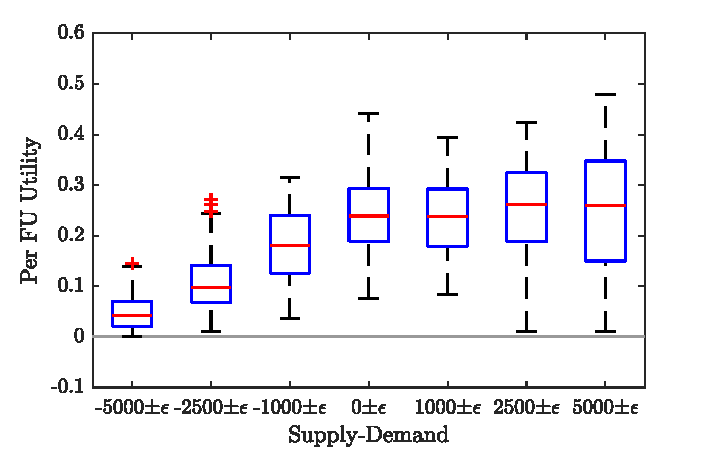
\includegraphics[width=\columnwidth]{Figures/PIMRC-fig2-a}%
% \caption{Buyers' Utility}%
% \label{PIMRC-fig2-a}%
% \end{subfigure}\hfill%
% \begin{subfigure}{.49\columnwidth}
% 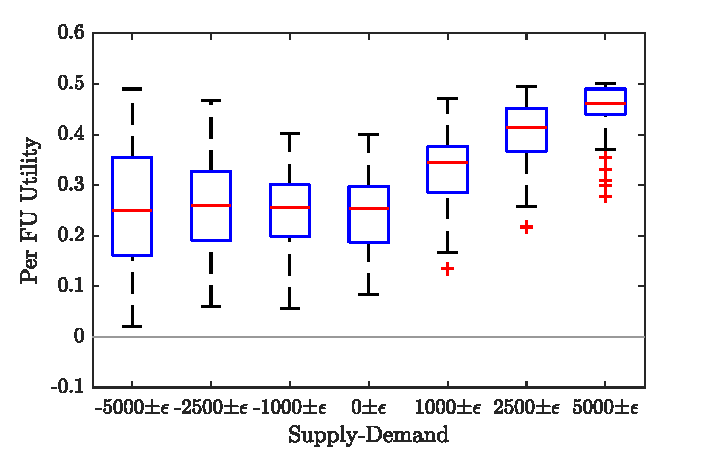
\includegraphics[width=\columnwidth]{Figures/PIMRC-fig2-b}%
% \caption{Sellers' Utility}%
% \label{PIMRC-fig2-b}%
% \end{subfigure}\hfill%
% \begin{subfigure}{.49\columnwidth}
% 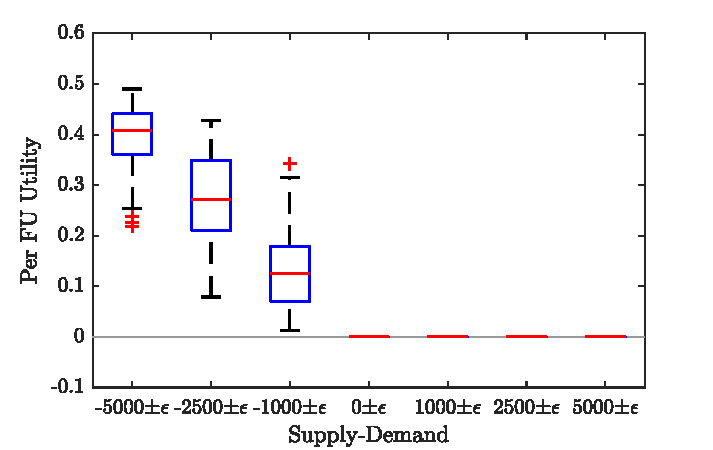
\includegraphics[width=\columnwidth]{Figures/PIMRC-fig2-c}%
% \caption{Inp's Utility}%
% \label{PIMRC-fig2-c}%
% \end{subfigure}%
% \caption{Market simulation results in various (Supply\textnormal{-}Demand) differences.
%   a) Buyers' Utility, b) Sellers' Utility, c) \ac{InP}'s Utility.}
%   \label{PIMRC-fig2}
% % \vspace{-7mm}
% \end{figure}
% \subsection{Results}
% In this section, we report the results of the market simulation proving the achievement of the two important properties of auction namely \textit{individual rationality} and \textit{weak budget balance}.\newline

% We simulate a market with ten \acp{VNO} each with an equal share of the upstream bandwidth, i.e., 9,953.28-Mbps$\approx$1-Gbps. This translates to 972 blocks (16 bytes) or FUs per frame (125 $\mu s$) per VNO.
% Each \ac{VNO} is allowed to ask for up to twice its share of the frame, i.e., in the range $[0-1944]$. \acp{VNO} will generate an optimistic \ac{BMap} considering being allocated all their demanded extra FUs in case that they are buyers, and selling all their excess FUs in case that they are sellers. Then, after holding the auction if the outcome is different the merging engine (operated by the InP) will adjust the issued \ac{BMap} according to the items that each \ac{VNO} successfully has acquired or sold. This is important in order to eliminate the need for an extra round of communication between the \ac{InP} and the \acp{VNO} to announce the outcome of the auction.

% The valuation for each FU reflects the probability of the \ac{VNO} to have demand from its users for an FU. This valuation is done by the \ac{VNO}, and it is either based on the methods specified in the standard, i.e., traffic monitoring and the queue occupancy reports from the ONUs or new methods such as traffic forecasting \cite{7495169}. The valuation (demand probability) is between $[0, 1]$ for both the seller and buyer VNOs.

% A \ac{VNO} is a seller if it has excess frame share and has a valuation less than $BasePrice$ for each frame unit, i.e., sellers' valuation is in the range $[0, BasePrice)$. A \ac{VNO} is an eligible buyer if its valuation is higher than $BasePrice$, i.e., in the range $(BasePrice ,1]$.
% Note that we interpret the high valuation for an item as a sign that the buyer with the highest valuation is the least likely of the buyers to waste the frame unit. We set the $BasePrice$ to 0.5 in our simulation meaning that if a \ac{VNO} has a strictly smaller probability of utilizing the frame share, it will be willing to trade it for a higher value. The choice of 0.5 as the $BasePrice$ is to achieve a trade-off between the number of eligible sellers and buyers. A higher $BasePrice$ will lead to a smaller population of eligible buyers and a smaller $BasePrice$ will limit the potential population of the sellers. We simulated the market for a duration of 10 minutes, which involves auctioning 4,800,000 consecutive frames, each of 125 $\mu s$ duration.
% \begin{figure}[h]
% % \vspace{-5mm}
% \centering
%   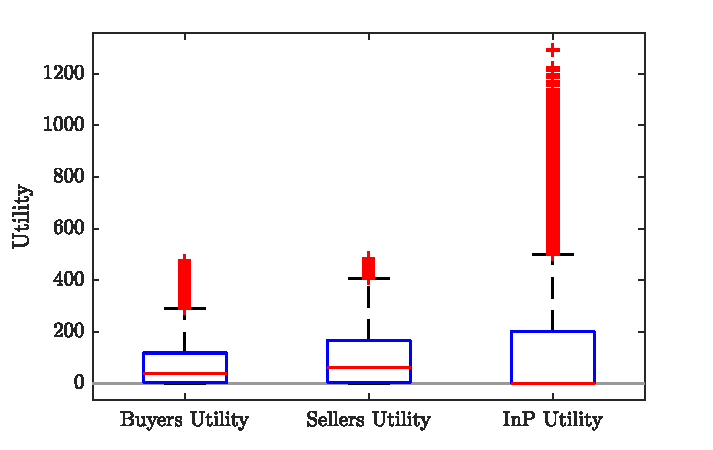
\includegraphics[scale =0.65]{Figures/PIMRC-fig3.pdf}
%   \caption{Market simulation results in total.}
%   \label{PIMRC-fig3}
% % \vspace{-8mm}
% \end{figure}

% The simulation results are illustrated in Fig.~\ref{PIMRC-fig2} and have been separated into three sub-figures based on the buyers', sellers' and \ac{InP}'s utility. In all sub-figures, the X-axis denotes the difference between the supply and demand ($Supply-Demand$). Each point in the X axis is a bin that contains the result of 100 auctions with a ($Supply-Demand$) difference falling within the range of $x\pm\epsilon$ when $\epsilon = 4$.

% To analyze the results statistically, we used \textit{box plots} for our numerical results. In a box plot, the quartiles of the data are shown graphically. The red line in the middle of the box is the median, and the lower and higher horizontal edges of the box denote the first and third quartile of the data, respectively. The dashed lines are the whiskers, and the red pluses are the outliers.


% Fig.~\ref{PIMRC-fig2-b} shows the box plots of the per FU utility of the buyers and the sellers. As expected in Fig.~\ref{PIMRC-fig2-a} we see that significantly lower supply than demand leads to a very low utility for buyers because the bid values are becoming very close to each other. So, the winner will pay a price which is very close to its valuation. The utility increases as the supply increases. While more supply than demand leads to higher average utility, it also means that all the bidders will pay the reserved price. This leads to a wide range of positive utilities for buyers; some will have high utility and others will have very low. This effect is visible on the right end of Fig.~\ref{PIMRC-fig2}.a. In Fig.~\ref{PIMRC-fig2}.b we see a similar effect on the left side where demand is much higher than supply. In Fig.~\ref{PIMRC-fig2}.c we present the utility of \ac{InP} which is non-zero only when the demand is higher than supply. For \ac{InP} $Supply-Demand\geq 0$ means that the buyers pay the reserved price which is equal to the procurement price from sellers. Thus, there is no revenue in these scenarios. On the other hand, \ac{InP} utility is positive when the demand is higher than supply.

% Finally, Fig.~\ref{PIMRC-fig3} represents the outcome of the auction throughout the whole duration of the simulation. Fig.~\ref{PIMRC-fig3} suggests that the system satisfies both \textit{individual rationality} and \textit{weak budget balance}, since the sellers', buyers', and \ac{InP}'s utility is never negative. Therefore, none of the \acp{VNO} nor the \ac{InP} will ever regret participating in the auction.
% \subsection{Conclusion}
% In this capter, we proposed an auction model to address the Inter-operator dynamic capacity sharing in virtualized multi-tenant PONs. The proposed auction mechanism is incentive compatible and satisfies all the desired economic properties. The auction was designed in a way to minimize any communication delay that could affect the network scheduling operations, which typically occur every 125 $\mu s$. For this purpose, \acp{VNO} send all the required information for conducting the auction at once, along with the \ac{BMap}. The market simulation results confirm our claim that our model is \textit{individual rational} and \textit{weak budget balanced}. These properties provide incentives for the seller \acp{VNO} to participate in the auction by selling their excess capacity and for the buyers to acquire it while implementing their desired bandwidth allocation mechanism. The \ac{InP} also benefits from the auction in two ways: first by receiving revenue for facilitating the auction; second, by operating the network resources more efficiently, which can lead to the possibility to accommodate a  higher number of \acp{VNO} in the same PON. A natural progression of this work is to analyze the effects of adjusting the $BasePrice$ according to the $Supply-Demand$ on the utilities of the sellers, buyers, and the InP.


% \subsection{VCG based auction and \acp{PON} utilization Results}
% To examine the impacts of different approaches toward sharing the \acp{PON} capacity, we compare three mechanisms:
% \begin{enumerate}
%   \item The "Non-Sharing" mechanism in which each \ac{VNO} gets its fixed share of the frame regardless of the demand;
%   \item The "Upper-Bound" mechanism in which the items from the cheapest sellers are sold to the highest offers for the reported values with a naive assumption of truthfulness (not economic-robust);
%   \item Our proposed "Economic-Robust Sharing" mechanism that facilitates the sharing through buying the items from the sellers for a fixed price of 0.5 and selling them to the buyers to the VCG price.
% \end{enumerate}
% We have simulated a multi-tenant \acp{PON} market considering a%\cite{G.9807.1}
% 10-Gbps symmetrical \acp{PON} (i.e., XGS-\ac{PON}). The simulation duration is 6 seconds, which allows us to average our results over 48,000 frames, each of 125 $\mu s$ duration. The \acp{PON} is shared amongst 10 VNOs, each serving 10 Optical network units (ONUs). Although not reported, we have repeated the same simulations for different numbers of ONUs and VNOs, obtained similar results.
% \begin{figure}[h]%
% % \vspace{-7mm}
% \centering
% \begin{subfigure}{.45\columnwidth}
% 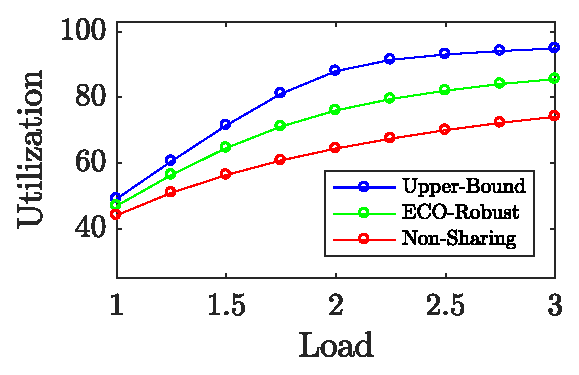
\includegraphics[width=\columnwidth]{Figures/ofc18-2}%
% \caption{Unbalanced Load}%
% \label{ofc18-2}%
% \end{subfigure}\hfill%
% \begin{subfigure}{.45\columnwidth}
% 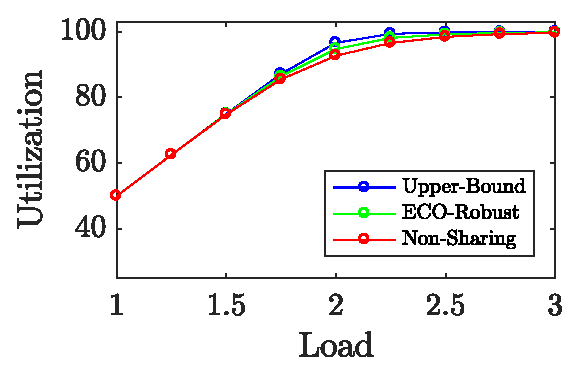
\includegraphics[width=\columnwidth]{Figures/ofc18-3}%
% \caption{Balanced Load}%
% \label{ofc18-3}%
% \end{subfigure}\hfill%
% \begin{subfigure}{.45\columnwidth}
% 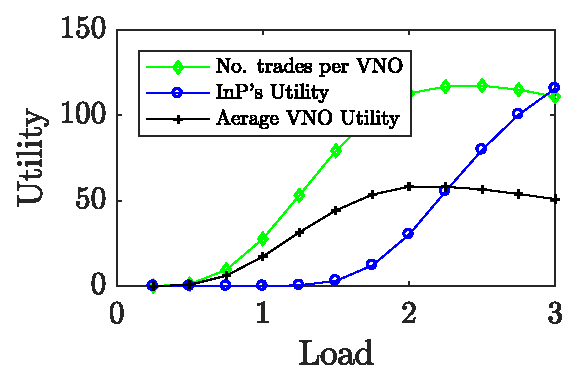
\includegraphics[width=\columnwidth]{Figures/ofc18-4}%
% \caption{Utility-Unbalanced Load}%
% \label{ofc18-4}%
% \end{subfigure}\hfill%
% \begin{subfigure}{.45\columnwidth}
% 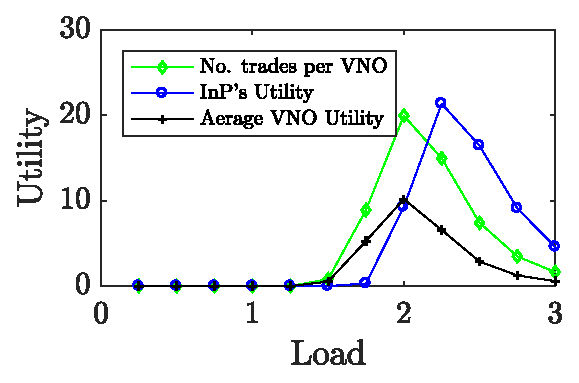
\includegraphics[width=\columnwidth]{Figures/ofc18-5}%
% \caption{Utility-Balanced Load}%
% \label{ofc18-5}%
% \end{subfigure}
% % \vspace{-5mm}
% \caption{Simulation results of our \ac{DBA} auctions, showing how the auction mechanism increases \acp{PON} utilization.}
%   \label{ofc18}
% % \vspace{-9mm}
% \end{figure}
% Our results are reported in \figureautorefname~\ref{ofc18}, comparing the three sharing mechanisms described above. \figureautorefname~\ref{ofc18-2} shows the network utilization for an unbalanced load scenario (i.e., the mean of the traffic generated by the ONUs is assigned according to a random uniform distribution), confirms that our proposed economic-robust mechanism outperforms the Non-Sharing by achieving higher utilization across all offered loads. The Upper-Bound scenario reflects the case that with no trade reduction and, as a result, it increases the number of trades, leading to higher utilization. It is important to note though that the upper-bound is idealistic since without incentivizing \acp{VNO} to report their truthful value, they will likely manipulate their bids to achieve higher utility: the buyer \acp{VNO} shading their bids, and the sellers reporting higher untruthful values. This leads to a higher price per item from the sellers and lower offer per item from buyers leading to a natural reduction of trades. However, our results do not account for the manipulative bidding behavior of the VNOs.
% In \figureautorefname~\ref{ofc18-3} we report, for completeness, the scenario with the balanced load across the ONUs, although this is less realistic. As expected, although the trend is confirmed, the difference between the three mechanisms is much less remarked, as the number and value of the trades are far less when \acp{VNO} all have similar traffic. \figureautorefname~\ref{ofc18-4} compares, for the unbalanced load scenario, the average VNOs' and \ac{InP}'s utility against the average number of trades conducted during each frame using the proposed mechanism.
% We define the VNOs' utility as the difference between their trading price and their valuation for the FU, .i.e., this determines how close is their final payment to their perceived value. The \ac{InP}'s utility is the difference between the trading price of the seller and buyer VNOs, i.e., this reflects the price gap occurred due to the supply and demand ratio.
% Both \figureautorefname~\ref{ofc18-4} and \figureautorefname~\ref{ofc18-5} show that as we move to the right along the X-axis, the ratio of the demand to supply increases and, as a natural reaction, the market adapts by raising the price. As the number of trades increases, \acp{VNO} and the \ac{InP} gain more utility. Once the overloading ratio exceeds the factor of 2, the \acp{VNO} become more demanding. At the same time, the supply declines and leads to fewer trades and eventually almost no trade when it reaches saturation as all the \acp{VNO} are asking for more than their negotiated share. By design, while the supply is higher than the demand the trading price is equal to the base price thus the utility of the \ac{InP} remains zero. Once the demand grows over the supply, the price rises and the \ac{InP}'s utility starts to grow. The \ac{InP}'s utility is at its highest when the number of trades is maximum, and the average price of an FU is high.

% To conclude, our work has shown that economic sharing incentives are indispensable in fully virtualized multi-tenant PONs to increase the overall utilization. Our proposed market mechanism significantly improves the utilization of the \acp{PON} compared to the Non-Sharing scenario while achieving the desired economic robustness.
% %%%%%%%%%%%%%%%%%%%%%%%%%%%%%%%%%%%%%%%%%%%%%%%%%%%%%%%%%%
% %%%%%%%%%%%%%%%%%%%%%%%%%%%%%%%%%%%%%%%%%%%%%%%%%%%%%%%%%%
% %%%%%%%%%%%%%%%%%%%%%%%%%SECTION%%%%%%%%%%%%%%%%%%%%%%%%%%
% %%%%%%%%%%%%%%%%%%%%%%%%%%%%%%%%%%%%%%%%%%%%%%%%%%%%%%%%%%
% %%%%%%%%%%%%%%%%%%%%%%%%%%%%%%%%%%%%%%%%%%%%%%%%%%%%%%%%%%
\section{McAfee-Based Double Auction Mechanism}
\label{sec:auction_mechanism}
We propose a sealed-bid homogeneous item double auction mechanism. In a sealed-bid auction all traders simultaneously submit sealed asks/bids to the auctioneer, and no trader is aware of the ask/bid of any other participant. An auction is a homogeneous item when the trading items are identical; thus the traders have no preferences over any of the items.


The mechanism provides a matching service to multiple buyers and sellers in a bilateral trade environment. We assume rational traders whose effort is focused on maximizing their payoff by trading the identical items. A market maker, or the auctioneer, is responsible for operating this market and conducting the auctions while having no or incomplete information about the true valuations of the traders. There is a finite number of alternative resource allocation combinations. Each combination would bring a different individual and social payoff for each trader and the entire market.
We chose a sealed-bid auction due to the latency constraints in \ac{PON} networks and the fact that we need to run the auction in microseconds time scales, we cannot afford multiple rounds of communication among the sellers, auctioneer and the buyers. Therefore, we have to minimize these communications. Using the sealed-bid version of auction helps us to eliminate the need for any additional round of communication among the agents as the traders only send the ask/bid values once along with their \ac{BMap} (the suggested allocation schedule). The algorithmic representation of the proposed double auction mechanism is given in \autoref{alg:MC_algorithm}.

\begin{algorithm}[htbp]
\DontPrintSemicolon
\SetAlgoLined
% \KwResult{Write here the result}
% \SetKwInOut{InPut}{InPut}\SetKwInOut{Output}{Output}
% \InPut{Write here the input}
% \Output{Write here the output}
\BlankLine
{Sort sellers ascending so $v^B_{1}>v^B_{2}>...>v^B_{m}$}
    \BlankLine
 {Sort buyers descending so $v^S_{1}<v^S_{2}<...<v^S_{n}$}
    \BlankLine
{Find $max(S_L, B_K) \ \forall \ v^{}_L<v^{}_K\ \textbf{and}$ \ {$\sum_{1}^\textsc{k} q_{j}^B \leq \sum_{1}^\textsc{l} q_{i}^S$}}{
    \BlankLine
    {$\gamma = {\frac{1}{2}}\times({v_\textsc{l+1}+v_\textsc{k+1}})$}
    }
    \BlankLine
  \uIf{$\gamma \in [{v^{}_L} , {v^{}_K}]$}{
		\BlankLine
         $\Theta^{}_{Pr} = \min (\sum_{1}^{i=L}{q_{i}}, \sum_{1}^{j=K}{q_{j}})$\;
        \BlankLine
        $p^B = p^S = \gamma$
        \BlankLine  }
  \uElseIf{$\gamma \notin [{v^{}_L} , {v^{}_K}]$}{
\BlankLine
         $\Theta^{}_{Pr} = \min (\sum_{1}^{i=L-1}{q_{i}}, \sum_{1}^{j=K-1}{q_{j}})$\;
        \BlankLine
        $p^B = v^{}_K$
        \BlankLine
        $p^S = v^{}_L$
        \BlankLine    }
\caption{Multi-Item Double Auction}
\label{alg:MC_algorithm}
\end{algorithm}

We assume that there are no restrictions on the sets of buyers and sellers that may trade with one another nor any preferences over trade between any of the traders. The steps of the proposed auction mechanism are as follows:
\begin{enumerate}
\item The auctioneer sorts all the buyers (based on their ask/bid value) so that:
\begin{equation}
\{\tilde{\mathbf{S}} = \{s_{1}, s_{2}, ...,s_{i}\} : v^S_{1}<v^S_{2}<...<v^S_{n}\}
\label{sorted_s}
\end{equation}
and
\begin{equation}
\{\tilde{\mathbf{B}} = \{b_{1}, b_{2}, ...,b_{j}\} : v^B_{1}>v^B_{2}>...>v^B_{m}\}
\label{sorted_b}
\end{equation}
\autoref{sorted_s} shows the sellers arranged in an ascending order and \autoref{sorted_b} shows the buyers sorted in a descending order by the value of their $v$.

\begin{figure}[htbp]%
% \vspace{-7mm}
\centering
\begin{subfigure}{0.85\columnwidth}
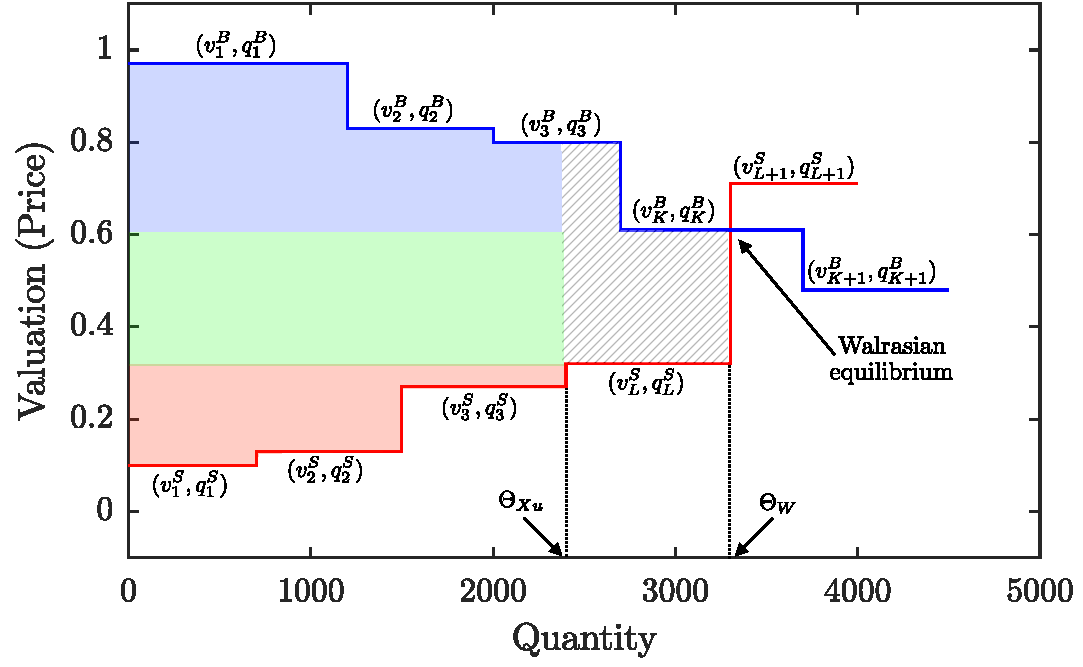
\includegraphics[width=\columnwidth]{Figures/sd_XU.pdf}%
\caption{\textit{Xu et al. \cite{5462277}} Double Auction}%
\label{sd_xu}%
\end{subfigure}\hfill%
\begin{subfigure}{0.85\columnwidth}
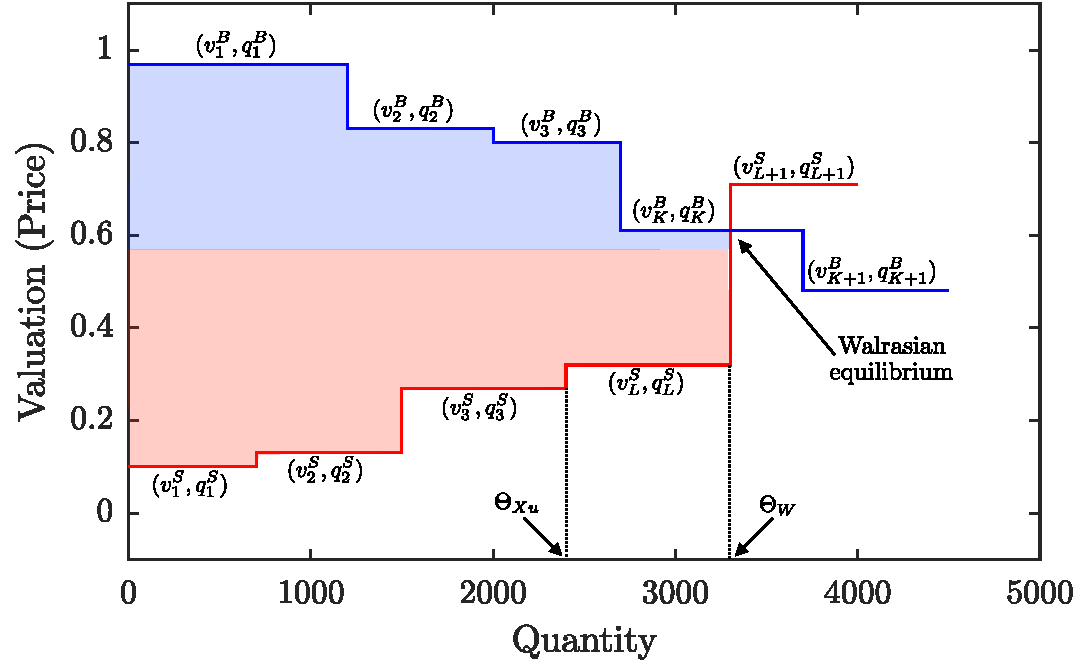
\includegraphics[width=\columnwidth]{Figures/sd_proposed.pdf}%
\caption{Proposed Double Auction}%
\label{sd_proposed}%
\end{subfigure}\hfill%
\caption{Discrete supply-demand graph of the double auction}
\label{sd}%
% \vspace{-6mm}
\end{figure}

\item The auctioneer discovers the Walrasian equilibrium quantity as shown in \figureautorefname~\ref{sd} as $\Theta_\textsc{w}$. \figureautorefname~\ref{sd_proposed} depicts the discrete supply and demand graph for one instance of the proposed auction (one round of the auction for one frame of the \ac{PON}) representing the trades' valuation and quantity. In \figureautorefname~\ref{sd} each step in the red line represents a seller, and each step in the blue line a buyer. In this example there are five sellers and five buyers in the market and $\gamma \in [{v^{}_L} , {v^{}_K}]$. As shown in \figureautorefname~\ref{sd_xu}, the gray area, representing the trading utility, is sacrificed to achieve truthfulness. In contrast, our proposed trade reduction technique depicted in \figureautorefname~\ref{sd_proposed} saves this amount of wasted utility while maintaining the truthfulness. In \figureautorefname~\ref{sd_xu}, the blue, green and red area represent buyers', auctioneer's and the sellers' utility from the auction. As it can be seen in \figureautorefname~\ref{sd_proposed}, for this particular instance of the market our proposed mechanism brings zero utility for the auctioneer. In general however, the auctioneer's overall utility will be the surplus between buyers' payment and the sellers' receivables goes to the auctioneer (zero when $\gamma \in [{v^{}_L} , {v^{}_K}]$ and $(p^\textsc{b} - p^\textsc{s}) \times \Theta$ when $\gamma \notin [{v^{}_L} , {v^{}_K}]$).



% Nevertheless, this does not mean that the auctioneer's overall utility will be zero as in the instance that $\gamma \notin [{v^{}_L} , {v^{}_K}]$ the surplus between buyers' payment and the sellers' receivables goes to the auctioneer.

\begin{Definition}
\textbf{Walrasian (Competitive) Equilibrium}

In the context of our double auction market, the ``Walrasian Equilibrium'' is the point in the supply-demand plot in which the supply equals the demand. This point specifies the maximum quantity of feasible trades in which the sellers' price is less than the buyers' price. In other words, this is the \textit{upper-bound} utilization of the market.
\end{Definition}

The Walrasian equilibrium defines another important factor, the ``Walrasian Price'' which, if the trade is conducted brings positive payoff for both the supplier and the demander and also balances the budget. i.e., it finds the biggest $(L, K)$ in which:
% \begin{equation}
% v_\textsc{l+1}\geq v^{}_K \geq v^{}_L, \textnormal{and} \sum_{1}^{K-1} q_{j}^B \leq \sum_{1}^\textsc{l} q_{i}^S \leq \sum_{1}^\textsc{k} q_{j}^B
% \end{equation}
% or
% \begin{equation}
% v^{}_K\geq v_\textsc{l+1} \geq v_\textsc{k+1}, \textnormal{and} \sum_{1}^{L-1} q_{i}^S \leq \sum_{1}^\textsc{k} q_{j}^B \leq \sum_{1}^\textsc{l} q_{i}^S
% \end{equation}

\begin{equation}
v^{B}_K\geq v^{S}_L \ \textit{and} \ v^{B}_{K+1} \leq v^{S}_{L+1},
\end{equation}
\vspace{-1mm}
and
\vspace{-1mm}
\begin{equation}
\sum_{j=1}^\textsc{k} q_{j}^B \leq \sum_{i=1}^\textsc{l} q_{i}^S.
\end{equation}
Thus the last trading seller and buyer in the walrasian equilibrium are called $S_L , B_K$ respectively.
The Walrasian equilibrium realizes the \textit{Pareto efficiency}. A resource allocation decision is referred to as Pareto efficient if it is impossible to reallocate the resources in a way that makes one of the agents better off without making others worse. This quality makes the Walrasian allocation a suitable benchmark of efficiency in economic analysis.


\item In order to achieve dominant strategy truthful value reporting we have to decouple the trade price of the sellers and buyers from their reported value. This is achievable through \textit{Trade Reduction}.

\begin{Definition}
\textbf{Trade Reduction}

A technique in which the least efficient trade in the market is sacrificed so the other traders can trade on their reported value, thus their reported valuation does not affect their payments, i.e., they have no incentive to report untruthful values (leading to \ac{IC}).
\end{Definition}
Thus, $q_{r}$ trades will be removed from the market. In \figureautorefname~\ref{sd_xu} the reduced area is shown in gray. Obviously, it is possible that by removing $q_{r}$ trades from the market we may have to eliminate more than two traders (completely or partially) from the market.

In our proposed mechanism, the total number of items sold by the sellers, which is equal to the total number of items bought, by the buyers is represented as $\Theta^{}_{Pr}$. The value of $\Theta^{}_{Pr}$ directly affects the utilization of the \acp{PON} link.
\vspace{-2mm}
\begin{equation}
\Theta^{}_{Pr} = \min (\sum_{i=1}^{L}{q_{i}}, \sum_{j=1}^{K}{q_{j}})
\end{equation}

The quantity of reduced trades is defined as $q^{}_R$:
\begin{equation}
q^{}_R = \Theta^{}_W - \Theta^{}_{Pr}
\end{equation}
The amount of efficiency (utility) sacrificed in market due to this trade reduction is:
\begin{equation}
\textit{Efficiency loss} = q^{}_R \times (v^{}_K-v^{}_L)
\end{equation}

% \textcolor{red}{MIDA and Hong \cite{5462277} stop here.
% }
\autoref{tbl:sd:RAW} presents the numerical information (the traders' preferences) used in \figureautorefname~\ref{sd_xu} and the different market results using the auction mechanism introduced by \textit{Xu et al.} \cite{5462277} (in \autoref{tbl:sd:XU}) and the results from the proposed mechanism in\autoref{tbl:sd:PROPOSED}.

\begingroup
\setlength{\tabcolsep}{2pt} % Default value: 6pt
\renewcommand{\arraystretch}{1} % Default value: 1

\newcolumntype{L}[1]{>{\raggedright\let\newline\\\arraybackslash\hspace{0pt}}m{#1}}
\newcolumntype{C}[1]{>{\centering\let\newline\\\arraybackslash\hspace{0pt}}m{#1}}
\newcolumntype{R}[1]{>{\raggedleft\let\newline\\\arraybackslash\hspace{0pt}}m{#1}}

\begin{table}
\caption{One Instance of the Double Auction Market.}\label{tbl:main}
\centering
\begin{subtable}[t]{\textwidth}
\centering
\vspace{0pt}
\begin{tabular}{|L{2cm}|C{2cm}|C{2cm}|C{2cm}|C{2cm}|L{1.8cm}|}
\hline
Sellers & 700@0.10  & 800@0.13 & 900@0.27 & 900@0.32 & 700@0.71 \\\hline
Buyers  & 1200@0.97 & 800@0.83 & 700@0.80 & 1000@0.61 & 800@0.48 \\ \hline
\end{tabular}
\vspace{3pt}
\caption{Sellers and buyers and their quantity to sell/buy@ask/bid price}
\label{tbl:sd:RAW}
\end{subtable}

\centering
\begingroup
\setlength{\tabcolsep}{2pt} % Default value: 6pt
\renewcommand{\arraystretch}{1} % Default value: 1
\begin{subtable}[t]{\textwidth}
\centering
% \vspace{7pt}
\begin{tabular}{|L{2cm}|C{2cm}|C{2cm}|C{2cm}|C{2cm}|L{1.8cm}|}
\hline
Sellers & 700@0.32  & 800@0.32 & 900@0.32 & 0 & 0 \\ \hline
Buyers  & 1200@0.61 & 800@0.61 & 400@0.61 & 0 & 0 \\ \hline
\multicolumn{1}{c}{} & \multicolumn{1}{c}{} & \multicolumn{1}{c}{} & \multicolumn{1}{c}{} &  &$\Theta= 2400$ \\ \cline{6-6}
\end{tabular}
\caption{Sellers and buyers and $\theta_i^S/\theta_j^B@p^S/p^B$ Xu et al. mechanism}
\label{tbl:sd:XU}

\end{subtable}
\endgroup

\centering
\begingroup
\setlength{\tabcolsep}{2pt} % Default value: 6pt
\renewcommand{\arraystretch}{1} % Default value: 1
\begin{subtable}[t]{\textwidth}
\centering
\vspace{0pt}
\begin{tabular}{|L{2cm}|C{2cm}|C{2cm}|C{2cm}|C{2cm}|L{1.8cm}|}
\hline
Sellers & 700@0.595  & 800@0.595 & 900@0.595 & 900@0.595 & 0 \\ \hline
Buyers  & 1200@0.595 & 800@0.595 & 700@0.595 & 600@0.595 & 0 \\ \hline
\multicolumn{1}{c}{} & \multicolumn{1}{c}{} & \multicolumn{1}{c}{} & \multicolumn{1}{c}{} &  &$\Theta= 3300$ \\ \cline{6-6}
\end{tabular}
\caption{Sellers and buyers and $\theta_i^S/\theta_j^B@p^S/p^B$ proposed mechanism}
\label{tbl:sd:PROPOSED}
\end{subtable}
\endgroup
\label{tbl:sd}
% \vspace{-7pt}
\end{table}
\endgroup
% \vspace{-4mm}

Our contribution in this chapter is to try and minimize $q^{}_R$ without loosing the economic properties. We use the technique used in \cite{MCAFEE1992434} which uses the values of $S_{L+1}$ (the strongest non-trading seller) and $B_{K+1}$ (the strongest non-trading buyer) to determine the traders payment only and only if:
\begin{equation}
\gamma = {\frac{1}{2}}\times({v_{{L+1}}^{S}+v_{{K+1}}^B}) \in [v_{i}^{S},v_{j}^{{B}}]
\end{equation}
thus since $v_L^S, v_K^B$, and in general none of the trading players, do not play a role in the price determination, i.e., there is no need to eliminate any of the traders including $S_{L}$ and $B_{K}$ from the market, therefore $q^{}_R = 0$. In this case the sellers and the buyers both trade in $\gamma=p^S=p^B$.

% If $\gamma \in [v_{i}^{\textsc{s}}, v_{j}^{\textsc{b}}]$:
% p^\textsc{b} =

\begin{Definition}
Weakest/Strongest Trader:
In the context of market power, the weakest traders are the seller with the highest asking price $v_{i}^S$ and the buyer with the lowest bid $v_{j}^{B}$. On the other side, strongest traders are the seller with the lowest ask and the buyer with the highest bid.
\end{Definition}

% \item If NOT 4 then we reduce the trades by removing  $S_L$ , $B_K$ from the trade and let other sellers and buyer trade in $P_\textsc{l}$ , $P_\textsc{k}$ respectively. (obviously, sometimes we need to, e.g.,remove multiple sellers in return for a single buyer vice-versa).
In Fig.\ref{sd_xu} the blue area is the sellers' utility, the green area is the auctioneer's and the red is the buyers'. The gray area is the amount of lost efficiency, e.g., when the trade reduction is applied.
\end{enumerate}

In the next section, we will provide the theoretical proofs for the economic robustness (see \autoref{Method:subsec:Economic-Robustness}) of the proposed auction mechanism.
% We consider an XGS-PON \cite{G.9807.1} with 10-Gbit/s symmetrical capacity in both upstream and downstream. We define the item to be traded in the auction as the most granular frame unit FU in an XGS-PON. This means for an upstream line rate of 9.953,28-Gbit/s each FU is one block (16 bytes) according to the XGS-PON standard. Thus, each XGS-PON frame (125 microseconds) can at most contain 9720 allocation structures. i.e., 9,720 FUs per frame.
% We consider a set of traders
% We consider a double auction in which allow for selling and buying excess frame units.


% We assume both the buyers' volume and the sellers' volume are drawn from a uniform distribution
% .


% \begin{figure*}%
% \centering
%   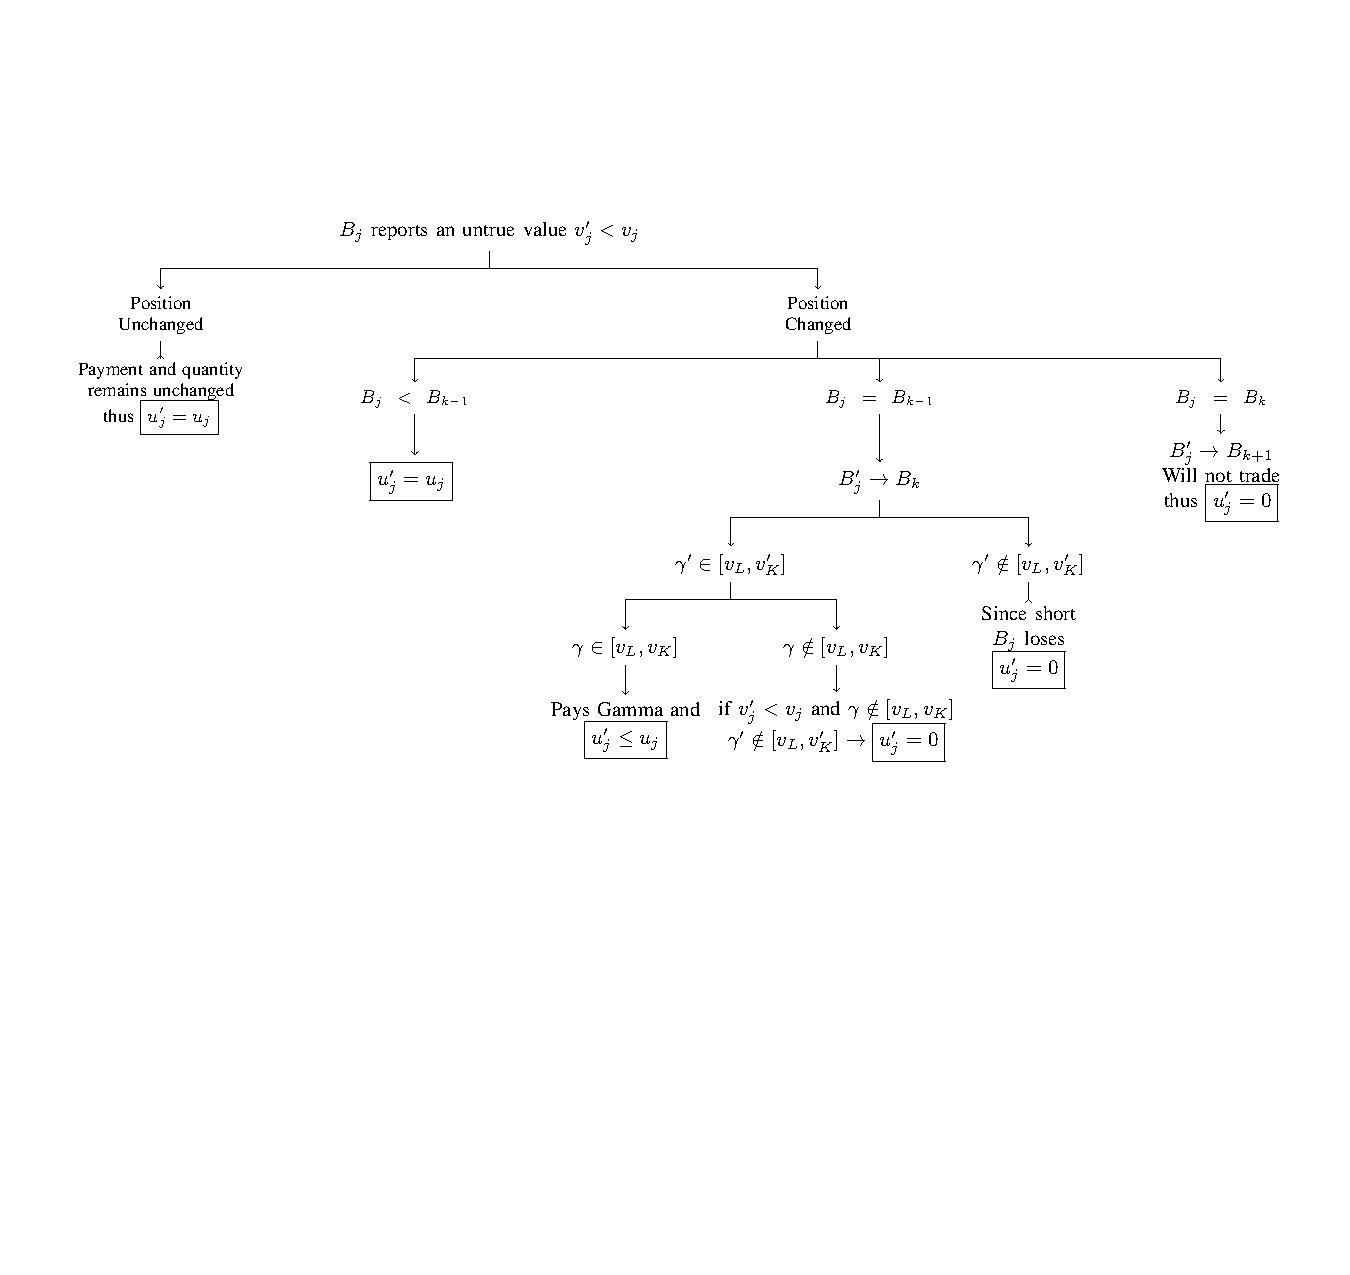
\includegraphics[width=1.9\columnwidth]{proof.pdf}
% \caption{Truthful Reporting dominant strategy proof}
%   \label{truth-proof}
% \end{figure*}
%%%%%%%%%%%%%%%%%%%%%%%%%%%%%%%%%%%%%%%%%%%%%%%%%%%%%%%%%%
%%%%%%%%%%%%%%%%%%%%%%%%%%%%%%%%%%%%%%%%%%%%%%%%%%%%%%%%%%
%%%%%%%%%%%%%%%%%%%%%%%%%SECTION%%%%%%%%%%%%%%%%%%%%%%%%%%
%%%%%%%%%%%%%%%%%%%%%%%%%%%%%%%%%%%%%%%%%%%%%%%%%%%%%%%%%%
%%%%%%%%%%%%%%%%%%%%%%%%%%%%%%%%%%%%%%%%%%%%%%%%%%%%%%%%%%
\section{Theoretical Proofs} \label{proofs}
\subsubsection{\acf{IC} or Truthfulness}
We have to prove that no trader can achieve higher utility by reporting a manipulated value which can be determined by market monitoring techniques and prediction tools such as machine learning etc.

% To prove this we have to prove that there is no ${v^\prime}^B_{j} < v^B_{j}$ which $B_{j}$ can report and by doing so gain more utility given that all the other bids and asks remain unchanged.

% \begin{Lemma}{Bid Independence:} $\nexists \ {{v^\prime}^B_{j} < v^B_{j}}\rightarrow ({u_{j}^\prime} \leq u_{j})$
% There is no ${v^\prime}^B_{j} < v^B_{j}$ which $B_{j}$ can report and by doing so gain more utility (${u_{j}^\prime} \leq u_{j}$) given that all the other bids and asks remain unchanged.
% \end{Lemma}

% \begin{proof}
% if $B_{j}$ reports a value ${v^\prime}^B_{j} < v^B_{j}$ there are two cases possible:
% \begin{itemize}
%     \item[] \textbf{Case a.} ${v^\prime}^B_{j}$ does not change the position where $B_{j}$ stands in the sorted buyer's list. In this case $B_{j}$ remains unchanged and its utility remains the same (${u_{j}^\prime} = u_{j}$).
%     \item[] \textbf{Case b.} ${v^\prime}^B_{j}$ changes the position where $B_{j}$ stands in the sorted buyer's list.
%     \begin{itemize}
%         \item[] \textbf{Case b.1} $\{B_{j^\prime}|j^\prime \leq k-1\}$: $B_{j}$ still wins all its demanded items, thus : ${u_{j}^\prime} = u_{j}$.
%         \item[] \textbf{Case b.2} $\{B_{j^\prime}|j^\prime = k\}$:
%         \begin{itemize}
%             \item[] \textbf{Case b.2.1} $\gamma^\prime \in [{v_{L}} , {v_{K}^\prime}]$:
%             \begin{itemize}
%                 \item[] \textbf{Case b.2.1.1} $\gamma \in [{v_{L}} , {v_{K}}]$: $B_{j}$ Pays Gamma Thus $u^\prime_{j} \leq u_{j}$.

%                 \item[] \textbf{Case b.2.1.2} $\gamma \notin [{v_{L}} , {v_{K}}]$: $B_{j}$ does not trade thus ${u_{j}^\prime} = 0$.

%             \end{itemize}
%             \item[] \textbf{Case b.2.2} $\gamma^\prime \notin [{v_{L}} , {v_{K}^\prime}]$: $B_{j}$ does not trade thus ${u_{j}^\prime} = 0$.

%         \end{itemize}
%     \end{itemize}
%     \item[] \textbf{Case b.3} $\{B_{j^\prime}|j^\prime = k+1\}$: $B_{j}$ still wins all its demanded items, thus : ${u_{j}^\prime} = 0$.
% \end{itemize}


% Reports lower untrue value and still wins the same quantity.
% Reports lower untrue value and wins a smaller number of items.
% Reports lower untrue value and loses.

% \end{proof}

\begin{Lemma}
\label{lemmaq}
No buyer can win more items by reporting an untruthfully lower value i.e., $\{\forall \ v^\prime_j < v_j | \theta^\prime_{j} \leq \theta_{j} \}$.
\end{Lemma}
\begin{proof}
The value of the $\theta^\prime_j$ depends on whether if the $v^\prime_j$ changes the position of $B_j$ in the sorted buyers' list.
\begin{itemize}
    \item[] \textbf{Case \ref{lemmaq}.a} If $B_j$ reports a $v^\prime_j < v_j$ and by doing so its position in the sorted buyers list does not change then by design the outcome of the auction remains the same. Therefore, the quantity will not change i.e., (${\theta_{j}^\prime} = \theta_{j}$).
    \item[] \textbf{Case \ref{lemmaq}.b} If the reported $v^\prime_j$ changes the position of the buyer in the sorted buyers list, since its position will be downgraded the $\theta^\prime_{j}$ at best case (e.g.,if $j \leq k$) will be equal to $\theta_{j}$ and in the worst case (e.g.,if $j=k+1$) zero i.e., ${\theta_{j}^\prime} \leq \theta_{j}$.


Thus we have proven that if $B_j$ reports an untruthful bid $v^\prime_j < v_j$ it cannot increase its trade quantity, i.e., $\nexists \ {{v^\prime}^B_{j} < v^B_{j}}\rightarrow ({\theta_{j}^\prime} \leq \theta_{j})$.
\end{itemize}
\end{proof}
\vspace{-5mm}
The game tree for this proof is depicted in \autoref{fig-proof-q}.
\begin{figure}[htbp]
\centering
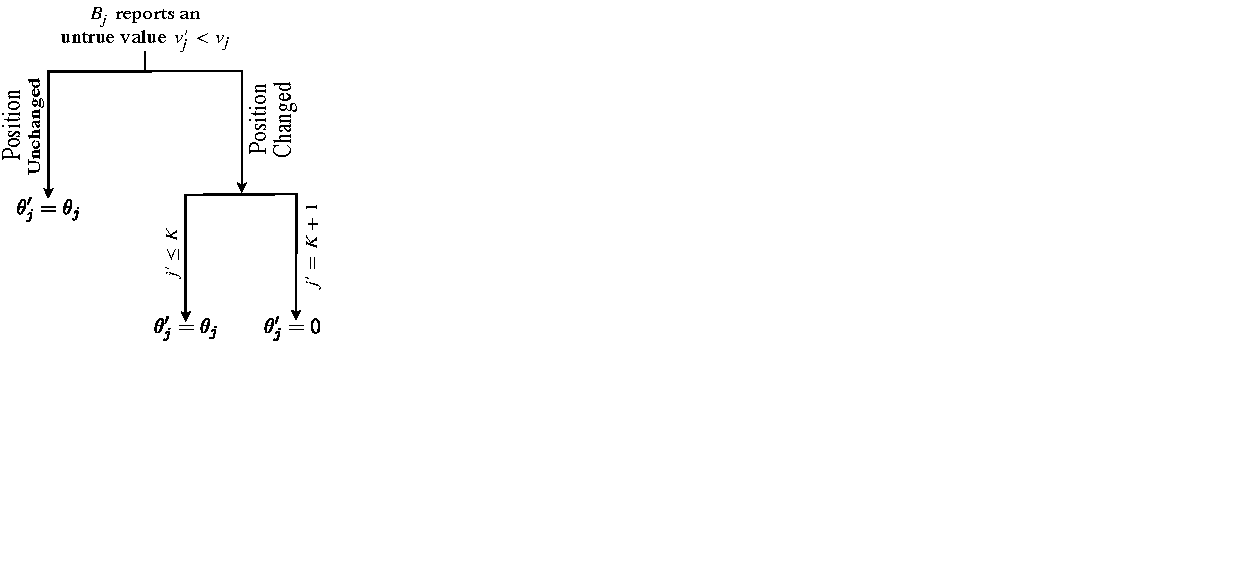
\includegraphics{Figures/proofq}
\caption{The proof tree for Lemma 1}
\label{fig-proof-q}
\vspace{-2mm}
\end{figure}
\begin{Lemma}
\label{lemma-p}
No buyer can decrease its per-item payment value by reporting an untruthfully lower value i.e., $\{\forall \ v^\prime_j < v_j | p^\prime_{j} \geq p_{j} \}$.
\end{Lemma}
\begin{proof}
Lets consider that $B_j$ reports an untruthful bid $v^\prime_j < v_j$.
\begin{itemize}
    \item[] \textbf{Case \ref{lemma-p}.a} If the new $v^\prime_j$ does not change the position of $B_j$ in the sorted buyers' list then the auction outcome remains unchanged, i.e., $p^\prime_{j} = p_{j}$.
    \item[] \textbf{Case \ref{lemma-p}.b} If the new $v^\prime_j$ does change the position of $B_j$ in the sorted buyers' list, the following cases can occur:
    \begin{itemize}
    \item[] \textbf{Case \ref{lemma-p}.b.1} If the new $j^\prime < K$ then the $p$ remains unchanged, i.e., $p^\prime_{j} = p_{j}$.
    \item[] \textbf{Case \ref{lemma-p}.b.2} If $j^\prime = K$ and $\gamma \in [{v^{}_L}, {v^{}_K}]$ then again $p^\prime_{j}$ remains unchanged as it is equal to $\gamma$ which is independent of the $v^\prime_j$, i.e., $p^\prime_{j} = p_{j}$.
    \item[] \textbf{Case \ref{lemma-p}.b.3} If $j^\prime = K$ and $\gamma \notin [{v^{}_L} , {v^{}_K}]$ then $B^\prime_j$ does not win any items, i.e., $p^\prime_j=0$.
    \item[] \textbf{Case \ref{lemma-p}.b.4} Finally if $j^\prime > K$ then $B^\prime_j$ does not win any items, i.e., $p^\prime_j=0$.
    \end{itemize}
\end{itemize}
Thus we have proven that if $B_j$ reports an untruthful bid $v^\prime_j < v_j$ it cannot lower its trade price, i.e., $\nexists \ {{v^\prime}^B_{j} < v^B_{j}}\rightarrow ({p^\prime_{j}} \leq p_{j})$.
\end{proof}
The game tree for this proof is depicted in \autoref{fig-proof-p}.
\begin{figure}[htbp]
% \vspace{-3mm}
\centering
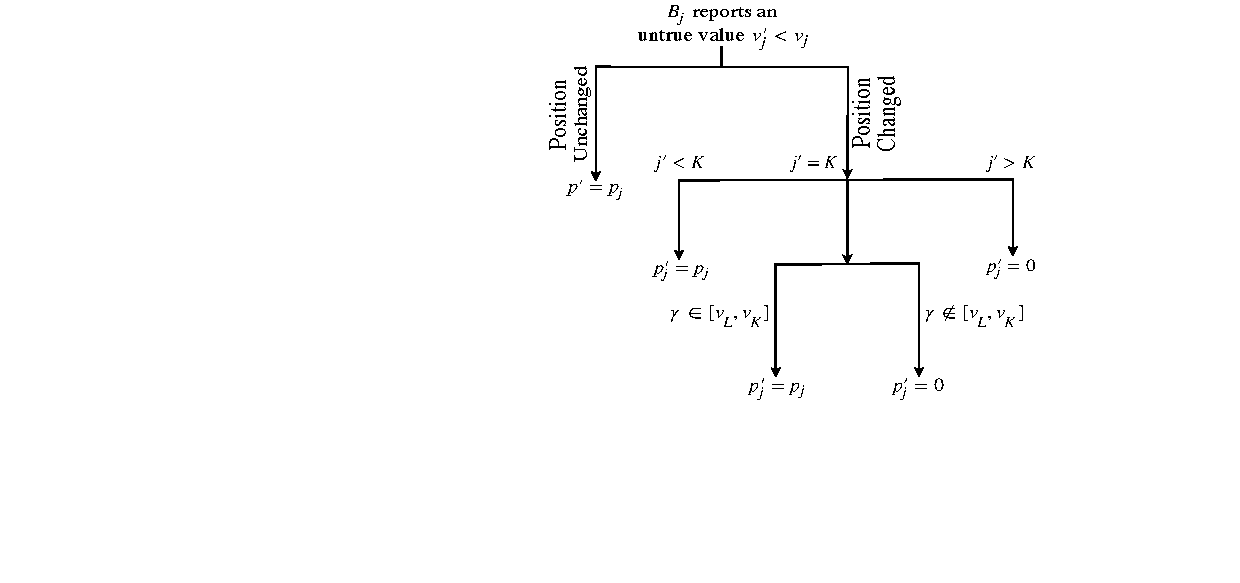
\includegraphics{Figures/proofp}
\caption{The proof tree for Lemma 2}
\label{fig-proof-p}
\vspace{-4mm}
\end{figure}
\begin{Theorem}\textbf{{Bid Independence:}} There is no ${v^\prime}^B_{j} < v^B_{j}$ which $B_{j}$ can report and by doing so gain more utility (${u_{j}^\prime} \leq u_{j}$) given that all the other players' bids and asks remain unchanged, i.e., $\nexists \ {{v^\prime}^B_{j} < v^B_{j}}\rightarrow ({u_{j}^\prime} \leq u_{j})$.
\label{Th-Bid-independence}
\end{Theorem}
\begin{proof}
According to \autoref{buyer-utility-formula} the utility of a buyer only increases if the quantity of trade increases or the price to pay decreases or both. By proving lemma~\ref{lemmaq} and lemma~\ref{lemma-p} we have proven that there is no way for any buyer to manipulate the market by reporting a lower value than its true valuation and gain higher utility by doing so, i.e., $\{\forall \ v^\prime_j < v_j | u^\prime_{j} \leq u_{j} \}$. Thus the final utility of a buyer is independent from the bid that it submits if not higher.
\end{proof}

\begin{Corollary}
According to theorem \ref{Th-Bid-independence}, the final utility is independent of the submitted bid. Thus it is a weakly dominant strategy for every buyer to report their true value and have a higher chance at winning since at worst the utility of truthful reporting is equal to that of a shaded (manipulated) bid.
\label{Corollary-buyers-truth}
\end{Corollary}
\begin{Corollary}
The dominant strategy truthfulness for the sellers can be proven in the same way as of Corollary \ref{Corollary-buyers-truth}.
\label{Corollary-sellers-truth}
\end{Corollary}

\subsection{Individual Rationality (IC)}
\begin{Theorem}
The proposed mechanism satisfies all traders' individual rationality.
\end{Theorem}
\begin{proof}
The proposed mechanism is \ac{IC} since by design it will not sell (buy) any item unless the trade price is higher (lower) than the seller's (buyer's) reported value. We consider that the \acp{VNO} are rational entities and would not report smaller values than their true value if they are sellers or bigger values than their true value if they are buyers.
\end{proof}

\subsection{Weak Budget Balance (BB)}
\begin{Theorem}
The proposed mechanism is BB.
\end{Theorem}
\begin{proof}
The suggested theorem is invalid when it is possible for the auctioneer to run a budget deficit. We will show that our mechanism does not allow that to happen.
According to \autoref{util-auc} to get a negative $u_{Auc}$ the following relationship must hold:
\begin{align*}
% u_{Auc}&<0
(p^\textsc{b} \times \sum_{1}^n {\theta_{j}^\textsc{b}}) &< (p^\textsc{s} \times \sum_{1}^m {\theta_{i}^\textsc{s}})
\end{align*}
that equivalently leads to the following inequality:
\begin{align*}
\frac{p^\textsc{b}}{p^\textsc{s}} &< \frac{\sum_{1}^n {\theta_{j}^\textsc{b}}}{\sum_{1}^m {\theta_{i}^\textsc{s}}}
\end{align*}
We know from the mechanism that $\sum_{1}^n {\theta_{j}^\textsc{b}}=\sum_{1}^m {\theta_{i}^\textsc{s}}=\Theta$, i.e., the total number of sold items is equal to the total number of items bought. Thus:
\begin{align*}
\frac{p^\textsc{b}}{p^\textsc{s}} &< 1 \qedhere
\end{align*}
According to our proposed mechanism, the buyers' trade price is always higher than the sellers' trade price, i.e., ${p^\textsc{b}}>{p^\textsc{s}}$. Therefore, the above inequality does not hold since it is in contradiction with the fact that ${p^\textsc{b}}>{p^\textsc{s}}$. Thus, we have proven that the $u_{Auc}$ can never be negative.
% For the following inequity to hold it is necessary that eq x which contradicts with our system design
% \begin{equation}
% (\sum_{1}^n {q_{j}^\textsc{b}}  \times p^\textsc{b}) < (\sum_{1}^m {q_{i}^\textsc{s}}  \times p^\textsc{s})
% \end{equation}
% We know from the mechanism that $P^B>P^S$, i.e., the buyers' trade price is always higher than the sellers' trade price. Thus it must hold that:
% \begin{equation}
% \frac{P^B}{P^S} < \frac{\sum_{1}^n {q_{j}^\textsc{b}}}{\sum_{1}^m {q_{i}^\textsc{s}}}
% \end{equation}
% \begin{equation}
% \frac{P^B}{P^S} < 1
% \end{equation}
% Which is in contradiction with the fact that $P^B>P^S$.
\end{proof}

% \begin{equation}
% min(\sum_1^{i={L-1}} q_i, \sum_1^{j={K-1}} q_j)\leq min(\sum_1^{i={L-1}} q_i, \sum_1^{j={K-1}} q_j) + \omega \times min(q_L,q_K)
% \mathbb{P}
% \end{equation}

% \begin{Theorem}
% The proposed mechanism has an acceptable allocative efficiency as it compares to the prior mechanisms.
% \begin{proof}

% \end{proof}
% \end{Theorem}
%%%%%%%%%%%%%%%%%%%%%%%%%%%%%%%%%%%%%%%%%%%%%%%%%%%%%%%%%%
%%%%%%%%%%%%%%%%%%%%%%%%%%%%%%%%%%%%%%%%%%%%%%%%%%%%%%%%%%
%%%%%%%%%%%%%%%%%%%%%%%%%SECTION%%%%%%%%%%%%%%%%%%%%%%%%%%
%%%%%%%%%%%%%%%%%%%%%%%%%%%%%%%%%%%%%%%%%%%%%%%%%%%%%%%%%%
%%%%%%%%%%%%%%%%%%%%%%%%%%%%%%%%%%%%%%%%%%%%%%%%%%%%%%%%%%
\section{Experimental Results} \label{results}
This section is dedicated to evaluating and analyzing the \ac{AE} of the proposed mechanism and comparing it to prior work. We measure the \ac{AE} by two factors:
\begin{enumerate}
\item The total number of items traded in one round of the auction (\autoref{Thetha}). This factor directly determines the proportion of the \acp{PON} bandwidth that is being shared among the VNOs. Thus it can clearly reflect the effect of auctioning the capacity on PON's efficiency.

To compare the results of different mechanisms we use the Walrasian equilibrium trade quantity as a baseline (upper-bound) since this is the maximum number of rational trades in the market. The closest the results are to the upper-bound the better. A rational trade is a trade in which the buyer's bid is strictly higher than the sellers, and the supply quantity is larger or smaller than the demand quantity.

\item The Social Welfare, which is a factor representing the aggregate benefit brought to all the parties involved in the market. The social welfare is calculated by summing the utilities of the trading traders and the auctioneer in every round of the auction. The social welfare can clarify whether the mechanism has been successful in redistributing the bandwidth from the sellers who value the items the least to the buyers with the highest valuation and therefore maximizing the total profit generated by the market. The Social Welfare is calculated as follows:

\begin{equation}
\label{SW:formula}
SW = \sum_{i=1}^{i=L} u^S_i + \sum_{j=1}^{j=K} u^B_j + u_{Auc}
\end{equation}
In which the SW is the social welfare of the system in each round of the auction.
\end{enumerate}


\subsection{Simulation Setup}
% In each second 9953280000 bits, in each second 8000 frames of 125 $\mu s$ and in each frame 9720 blocks each 16 bytes.
We consider an XGS-PON \cite{G.9807.1} with 10 Gbit/s (nominal line rate of 9.95328 Gbit/s symmetrical capacity). We simulate a market with ten \acp{VNO} each with an equal share of the upstream bandwidth, i.e., 995.328 Mbit/s$\approx$1-Gbit/s. This translates to 972 blocks (one block is 16 bytes as defined in the standard \cite{G.9807.1} as the finest granularity for upstream allocation) or blocks per frame (125 $\mu s$) per VNO.
Each \ac{VNO} will ask for a number of blocks depending on its users' instantaneous demand. This number determines that if the \ac{VNO} is a seller (if asking for a lower than the pre-defined share), a buyer (if asking for higher) or a non-trader (if asking for the exact same amount).

% The valuation for each FU reflects the probability of the \ac{VNO} to have a demand from its users for a FU. This valuation is done by the \ac{VNO}, and it is either based on the methods specified in the standard, i.e., traffic monitoring, and the queue occupancy reports from the ONUs or new methods such as traffic forecasting \cite{7495169}. The valuation (demand probability) is between $[0, 1]$ for both the seller and buyer VNOs.


\subsection{Simulation Results}
In this section, we report the market simulation results regarding Market Utility Distribution, Network utilization, and the Social welfare (see \autoref{Method:subsec:simul}). 


\subsubsection{Network Utilization}

\begin{figure}[h]
% \vspace{-7mm}
\centering
\begin{subfigure}{0.7\columnwidth}
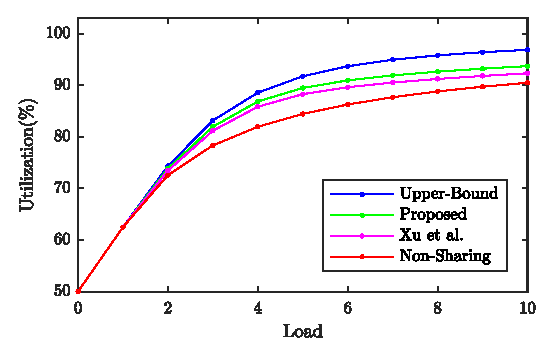
\includegraphics[width=\columnwidth]{Figures/fig1b}%
\caption{Unbalanced Load}%
\label{Unbalanced_Utilization}%
\end{subfigure}\hfill%
\begin{subfigure}{0.7\columnwidth}
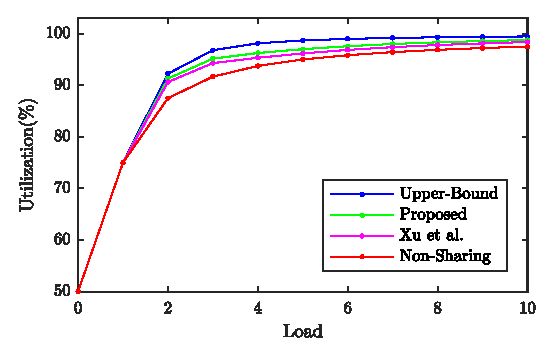
\includegraphics[width=\columnwidth]{Figures/fig1a}%
\caption{Balanced Load}%
\label{Balanced_Utilization}%
\end{subfigure}\hfill%
\caption{Simulation results of our \ac{DBA} auctions, showing how the auction mechanism increases \acp{PON} utilization.}
\label{Utilization}%
% \vspace{-9mm}
\end{figure}

\figureautorefname~\ref{Utilization} illustrates the performance comparison of the proposed mechanism with non-sharing and \textit{Xu et al.} \cite{5462277} mechanism. The \textit{"Upper-Bound"} is the maximum reachable utilization while overlooking the economic properties. As we mentioned in the previous sections "\textit{Xu et al.}" is a mechanism that works similar to our proposed mechanism with a difference that its trade reduction mechanism always removes $S_L , B_K$. The \textit{"Non-sharing"} represents the approach where \acp{VNO} do not share their excess capacity with others (i.e., no auction happens, and all the excess capacity is wasted).

Figures \ref{Unbalanced_Utilization} and \ref{Balanced_Utilization} depict the utilization (averaged over the simulation time) of each mechanism in the unbalanced (randomly weighted load) and balanced (equally weighted load) network loads respectively. Intuitively, the \textit{"Upper-Bound"} achieves the highest utilization as it ignores the truthfulness and puts a naive trust on the \acp{VNO} to report their values truthfully, thus does not remove any trades from the market. However, this is not acceptable since in such conditions the traders do not have any incentive to report true values and will potentially try to manipulate the market by reporting untrue values. This may lead to a situation where no trader gets to trade since they all are greedily trying to maximize their own utility without considering the others' welfare, e.g., ask prices are too high and bids are too low, so no trade happens. The horizontal axis in \autoref{Utilization} represents the average incoming load of each \ac{VNO}, and the vertical axis shows the utilization of each mechanism in a given load.

\begin{table}[htbp]
   \caption{Unbalanced Load Utilization}
   \label{tab:util:unbal}
   \small % text size of table content
   \centering % center the table
   \begin{tabular}{lcccccccr} % alignment of each column data
   \toprule[\heavyrulewidth]\toprule[\heavyrulewidth]
       Load & Non-Sharing    & \textit{Xu et al.} & Proposed    & Upper-Bound \\ \hline
   \midrule
    1  & 75.01  & 75.01 & 75.01 & 75.01\\
    2  & 87.51  & 90.64 & 91.28 & 92.24\\
    4  & 93.75  & 95.34 & 96.26 & 98.14\\
    6  & 95.84  & 96.86 & 97.58 & 99.00\\
    8  & 96.88  & 97.81 & 98.33 & 99.31\\
    10 & 97.51  & 98.38 & 98.77 & 99.47\\
   \bottomrule[\heavyrulewidth]
   \end{tabular}
\end{table}

\begin{table}[htbp]
   \caption{Balanced Load Utilization}
   \label{tab:util:bal}
   \small % text size of table content
   \centering % center the table
   \begin{tabular}{lcccccccr} % alignment of each column data
   \toprule[\heavyrulewidth]\toprule[\heavyrulewidth]
       Load & Non-Sharing    & \textit{Xu et al.} & Proposed    & Upper-Bound \\ \hline
   \midrule
    1  & 62.51  & 62.51 & 62.51  & 62.51\\
    2  & 72.59  & 73.46 & 73.86  & 74.35\\
    4  & 81.96  & 85.85 & 86.86  & 88.58\\
    6  & 86.28  & 89.63 & 90.96  & 93.70\\
    8  & 88.81  & 91.23 & 92.65  & 95.80\\
    10 & 90.49  & 92.33 & 93.72  & 96.88\\
   \bottomrule[\heavyrulewidth]
   \end{tabular}
\end{table}

The numerical results of the simulation are given in Table \ref{tab:util:unbal} and Table \ref{tab:util:bal}. According to our results, in both balanced and unbalanced load, the proposed mechanism outperforms \textit{Xu et al.} mechanism as its trade reduction technique allows more trades to be conducted.



% % % % % % % % % % % % % % % % % % % % 
% % % % % % % % % % % % % % % % % % % % 
% % % % % % %ACP Results % % % % % % % % 
% % % % % % % % % % % % % % % % % % % % 
% % % % % % % % % % % % % % % % % % % % 

\subsubsection{Market Utility Distribution}
The utility (profit) function of the sellers, buyers and the \ac{InP} are defined as $u_{i}^\textsc{s}$, $u_{j}^\textsc{b}$, and $u^{Auc}$.
% If the mechanism is \ac{IC} it means that we have access to the true valuation of the traders; thus it is possible to elicit the amount of utility they gain in the auction. 
The utility of a seller ($u_{i}^\textsc{s}$) is the difference between the per-item selling price and the asking price of that seller, times the number of items sold $\theta_{i}^\textsc{s}$:
\begin{equation}
\vspace{-1mm}
\label{seller_utility_formula}
u_{i}^\textsc{s} = {\theta_{i}^\textsc{s}}  \times (p^\textsc{s} - {v_{i}^\textsc{s}})
\end{equation}
Similarly for the buyers:
\begin{equation}
\vspace{-1mm}
\label{buyer_utility_formula}
u_{j}^\textsc{b} = {\theta_{j}^\textsc{b}}  \times ({v_{j}^\textsc{b}}-p^\textsc{b})
\end{equation}
The utility of the auctioneer is the difference between the amount paid by the buyers and the amount to be paid to the sellers:
% Hence:
\begin{eqnarray}
\vspace{-4mm}
u^{Auc} = (p^\textsc{b} - p^\textsc{s}) \times \Theta
\end{eqnarray}
 Where $\theta_{i}^\textsc{s}$ is the items sold by the $i^{th}$ seller for the price of $p^\textsc{s}$, ${\theta_{j}^\textsc{b}}$ is the items won by the $j^{th}$ buyer with the price of $p^\textsc{b}$, and $\Theta$ is the total number of items traded.

\begin{figure}[htbp]
% \vspace{-7mm}
\centering
\begin{subfigure}{0.7\columnwidth}
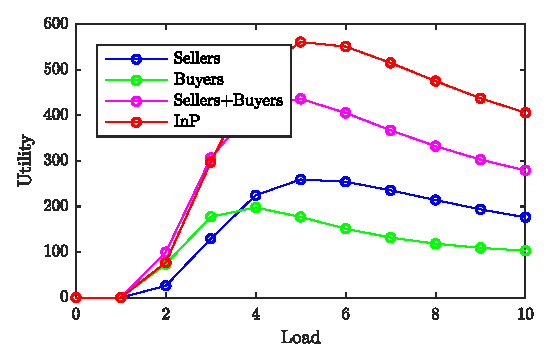
\includegraphics[width=\columnwidth]{Figures/U-Utility-s-b-traders.eps}%
\caption{Unbalanced}%
\label{fig:utility:unbalanced}%
\end{subfigure}\hfill%
\begin{subfigure}{0.7\columnwidth}
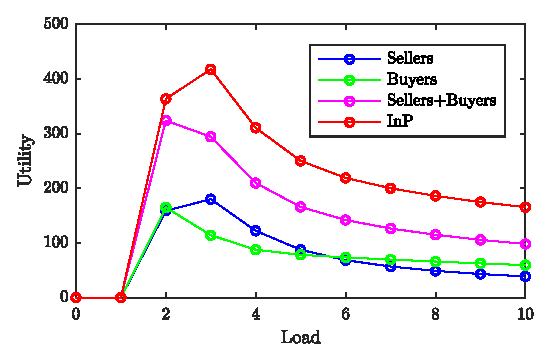
\includegraphics[width=\columnwidth]{Figures/B-Utility-s-b-traders.eps}%
\caption{Balanced}%
\label{fig:utility:balanced}%
\end{subfigure}\hfill%
\caption{Utility Distribution in the Marketplace}
\label{fig:utility}%
% \vspace{-3mm}
\end{figure}
\figureautorefname~\ref{fig:utility} shows the utility distribution between the trades and the InP. The utility of all the traders decline as the load saturates the network and the volume of offered capacity drops. Consequently, the total number of trades experiences reduction.


% % % % % % % % % % % % % % % % % % % % 
% % % % % % % % % % % % % % % % % % % % 
% % % % % % %ACP Results % % % % % % % % 
% % % % % % % % % % % % % % % % % % % % 
% % % % % % % % % % % % % % % % % % % % 


\subsubsection{Social Welfare}
\begin{figure}[htbp]%
% \vspace{-7mm}
\centering
\begin{subfigure}{0.7\columnwidth}
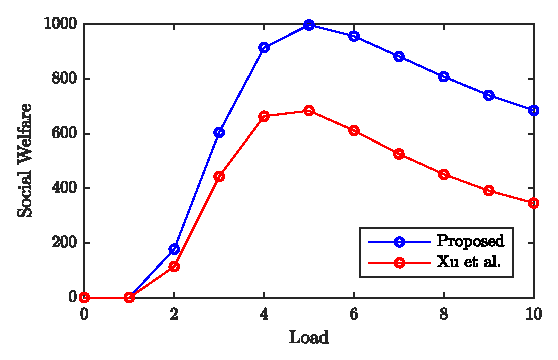
\includegraphics[width=\columnwidth]{Figures/fig1b-sw}%
\caption{Unbalanced Load}%
\label{sw:Unbalanced_Utility}%
\end{subfigure}\hfill%
\begin{subfigure}{0.7\columnwidth}
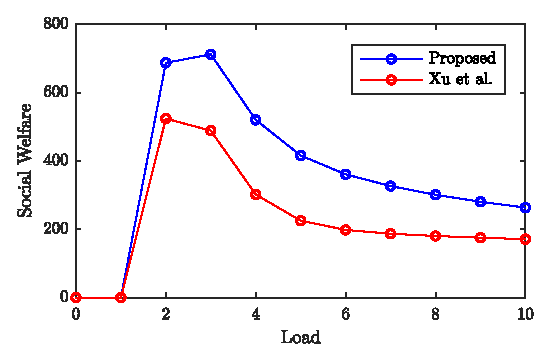
\includegraphics[width=\columnwidth]{Figures/fig1a-sw}%
\caption{Balanced Load}%
\label{sw:balanced_Utility}%
\end{subfigure}\hfill%
\caption{Simulation results of our \ac{DBA} auctions, showing how the auction mechanism increases the average Social Welfare.}
\label{Utility}%
% \vspace{-4mm}
\end{figure}


\figureautorefname~\ref{Utility} provides an insight into the social welfare (aggregate market utility averaged over the simulation time) generated by auctioning the excess capacity of the PON. The unit for utility is one block (XGS-PON frame block), e.g., the utility of 1000 in the \figureautorefname~\ref{sw:Unbalanced_Utility} means that on average over 10 seconds of simulation time $\approx1000$ additional frame blocks worth of utility is gained when using the proposed mechanism. The results in \figureautorefname~\ref{Utility} provides further support for the hypothesis that the proposed mechanism achieves higher social welfare compared to that of the Xu et al. \cite{5462277}. The explanation for this difference lays in our trade reduction technique that reduces fewer trades compared to the Xu et al. \cite{5462277}. We recognize that the significant improvements in \figureautorefname~\ref{sw:Unbalanced_Utility} that reaches up to $\approx 40\%$ may seem unrealistic at first glance. To explain this, it is important to note that as the network load increases, the number of eligible traders is reduced since it becomes less likely for a \ac{VNO} to have any excess resources to share. Therefore, it is likely that the trade eliminated by the trade reduction algorithm might be the only efficient trade, i.e., the trade reduction technique might ban the only feasible trade thus leaving the market with no additional social welfare.
% of zero. Therefore, our trade reduction will partly solve this problem by eliminating less efficient trades.

% \textcolor{brown}{To be mentioned in results analysis:
% }
% 1- As the load increases the \acp{VNO} are more likely to have a demand higher than their pre-allocated fixed capacity thus it is more probable to have higher number of buyers than sellers. The simulations are designed this way on purpose since we are more interested to observe the market in a high demand to supply ratio as this is more interesting compared to a high supply to demand ratio where the market is less competitive. This means that statistically since the bids and asks are uniform variables, in the competition between the buyers there is a higher chance for a high bid buyer to be present in the market leading to a higher average utility for the buyers' group, i.e., competition in the buyers' side increases linearly as the load increases.
% In figure unbalanced utility its visible that the number of trades increase as the load increase as the upper-bound for the load increases the probability of having buyers increases against having sellers. thus in each auction the probability of having sellers reduces.

% In figure balanced load utility the point in which the load is two, you can see the average per auction sellers' utility is equal to the buyers'. However, as we move to higher loads the

% \subsection{Different number of \acp{VNO} to show the efficiency grows}
%%%%%%%%%%%%%%%%%%%%%%%%%%%%%%%%%%%%%%%%%%%%%%%%%%%%%%%%%%
%%%%%%%%%%%%%%%%%%%%%%%%%%%%%%%%%%%%%%%%%%%%%%%%%%%%%%%%%%
%%%%%%%%%%%%%%%%%%%%%%%%%SECTION%%%%%%%%%%%%%%%%%%%%%%%%%%
%%%%%%%%%%%%%%%%%%%%%%%%%%%%%%%%%%%%%%%%%%%%%%%%%%%%%%%%%%
%%%%%%%%%%%%%%%%%%%%%%%%%%%%%%%%%%%%%%%%%%%%%%%%%%%%%%%%%%
\section{Conclusion} \label{auct:conclution}
In this chapter, We addressed one of the economic challenges facing the realization of \ac{PON} sharing. We provided an answer to the following research questions: 

\begin{itemize}
    \item \textit{\RQc}: We designed a market model for \ac{PON} excess capacity sharing, where multiple \acp{VNO} can engage in the trade of excess resources and receive monetary compensation for sharing their resources with other \acp{VNO}. The following will benefit from the proposed marketplace:
    \begin{itemize}
    \item The \acp{VNO} will be able to monetize their idle resources and also provide higher peak information rate (PIR) for their customers while reducing the risk of over-provisioning. %and for lower cost.
    \item The \ac{InP} can more efficiently utilize its infrastructure, allowing it to support more operators with no extra \ac{CapEx}.
    \item The end-users can enjoy more realistic information rates offered by the operators and reach a better quality of experience (QoE).
    \end{itemize} 
    
     \item \textit{\RQd}: We proposed a new sealed-bid, multi-item, double auction mechanism to efficiently allocate the resources while maximizing the social welfare of the market. The auction is designed in a way to minimize any communication delay that could affect the \ac{PON} scheduling operation, which typically occur every 125 $\mu s$. For this purpose, \acp{VNO} send all the required information for conducting the auction at once, along with the \ac{BMap}. We have proven that our proposed algorithm is compatible with the \acp{VNO}' incentives and guarantees positive a budget for the \ac{InP}. The results from the market simulation show that the proposed mechanism outperforms the state-of-the-art double auction mechanism proposed by Xu et al. \cite{5462277}, as our trade reduction mechanism scarifies fewer trades to achieve the crucial economic properties. Finally, these achievements are reached while the mechanism adds no additional communication overhead to the system due to its single-rounded nature.
\end{itemize}





\subsection{Peer-Reviewed Dissemination}

 \begin{enumerate}
   
    \item \textbf{\underline{N. {Afraz}}} and M.~{Ruffini}, ``A Sharing Platform for Multi-Tenant PONs,'' \emph{Journal of Lightwave Technology}, vol.~36, no.~23, pp. 5413--5423, Dec 2018.

    \item \textbf{\underline{N. {Afraz}}} and M.~{Ruffini}, ``A Marketplace for Real-Time Virtual PON Sharing,'' in \emph{2018 Asia Communications and Photonics Conference (ACP)}, Oct 2018, pp. 1--3.

    \item \textbf{\underline{N. {Afraz}}}, A.~{Elrasad}, M.~{Ruffini}, ``DBA Capacity Auctions to Enhance Resource Sharing Across Virtual Network Operators in Multi-Tenant PONs,'' in \emph{2018 Optical Fiber Communications Conference and Exposition (OFC)}, March 2018.
   
    \item \textbf{\underline{N. {Afraz}}}, A.~{Elrasad}, H.~Ahmadi,  M.~{Ruffini}, ``Inter-Operator Dynamic Capacity Sharing for Multi-Tenant Virtualized PON,'' in \emph{2017 IEEE 28th Annual International Symposium on Personal, Indoor, and Mobile Radio Communications (PIMRC)}, Oct 2017, pp. 1--6.

 \end{enumerate}
